\chapter{Supplementary Material}
\label{ch:Supplementary}

The following pages contain the supplementary material for this thesis. This section includes documents specific to project planning and management. The documents are attached in this order: \par

\begin{itemize}
    \item Project Assignment
    \item Risk Management
    \item Project Planning
\end{itemize}
\vspace{\baselineskip}
\noindent
Additionally, the appendix contains detailed information on the IQA databases from the general image domain, showcases the different dermatology quality criteria and their types across five severity ranges, and provides an overview of the proposed framework for automated IQA in teledermatology. \par

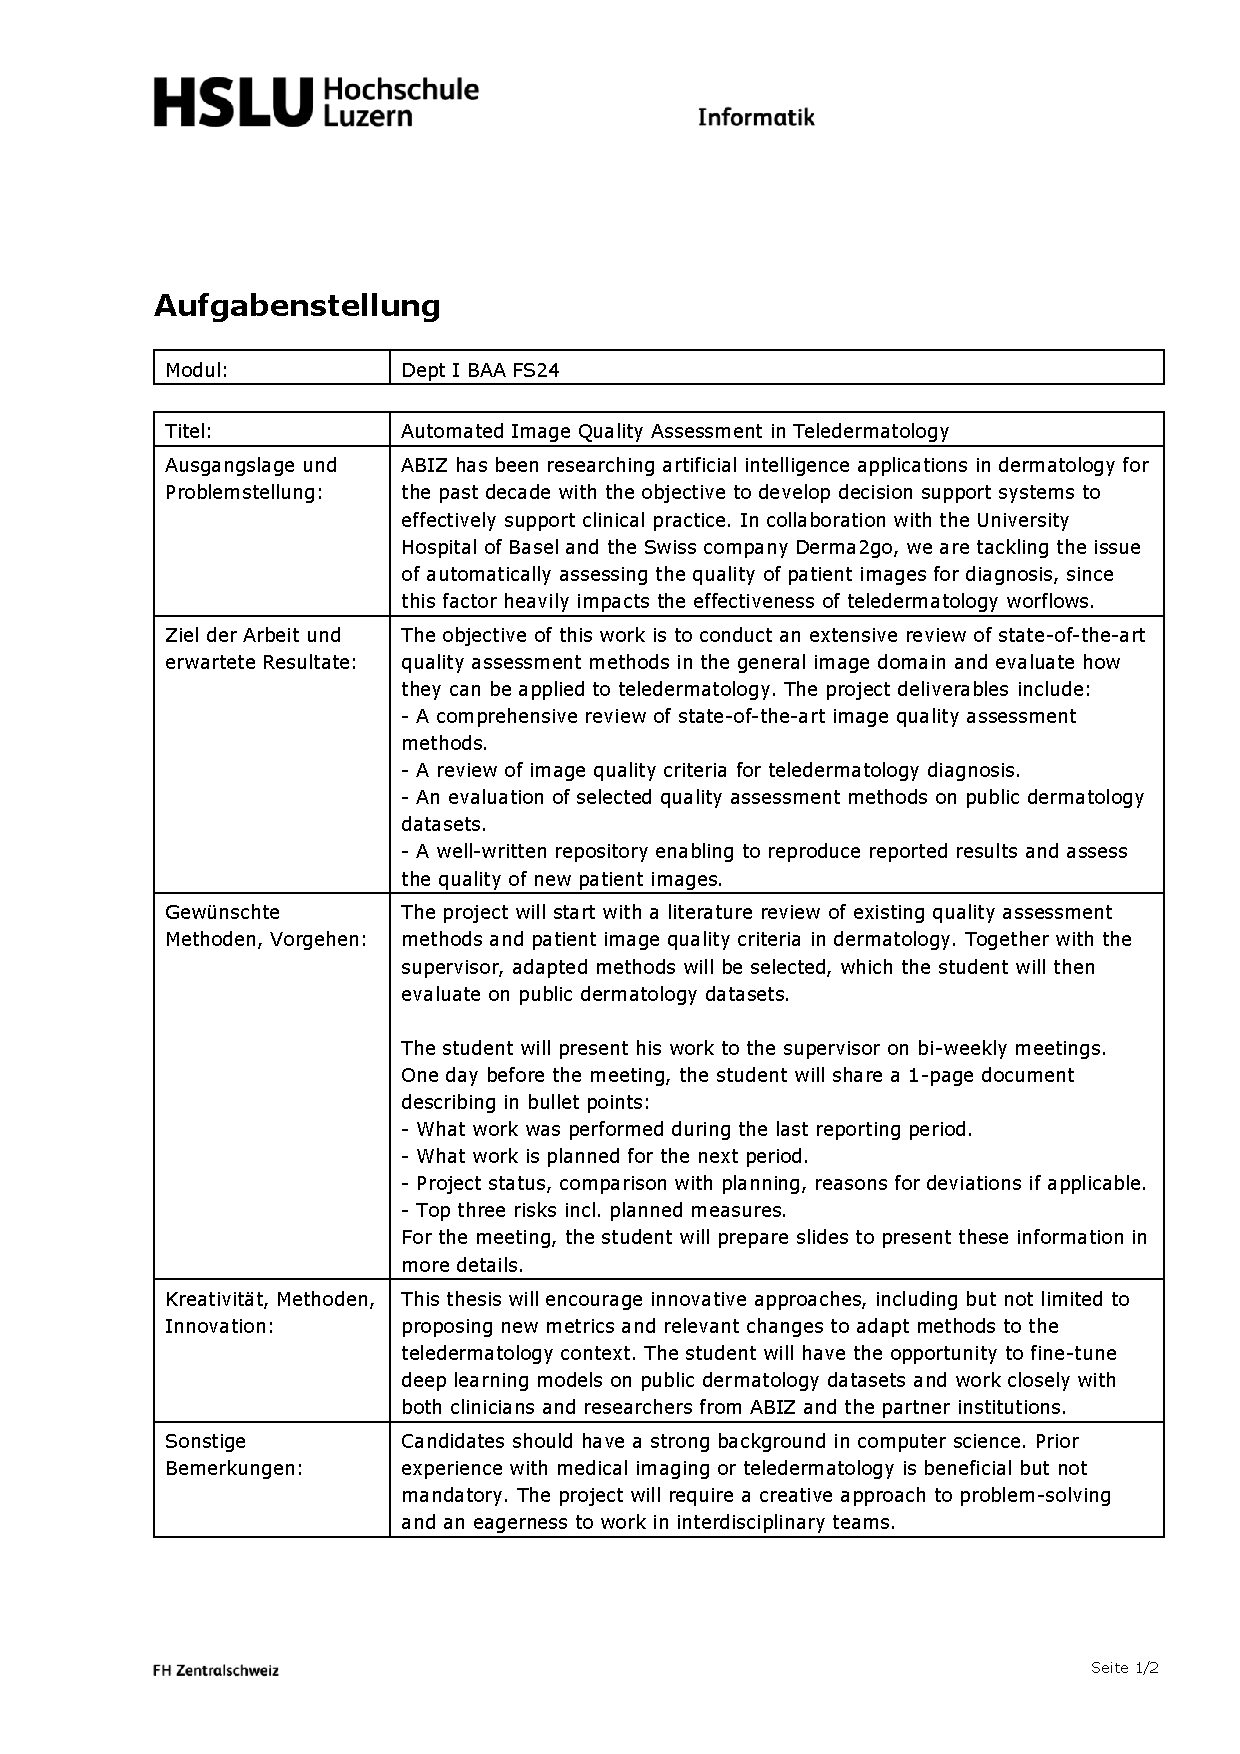
\includepdf[pages=-]{Aufgabenstellung_BAA.pdf}
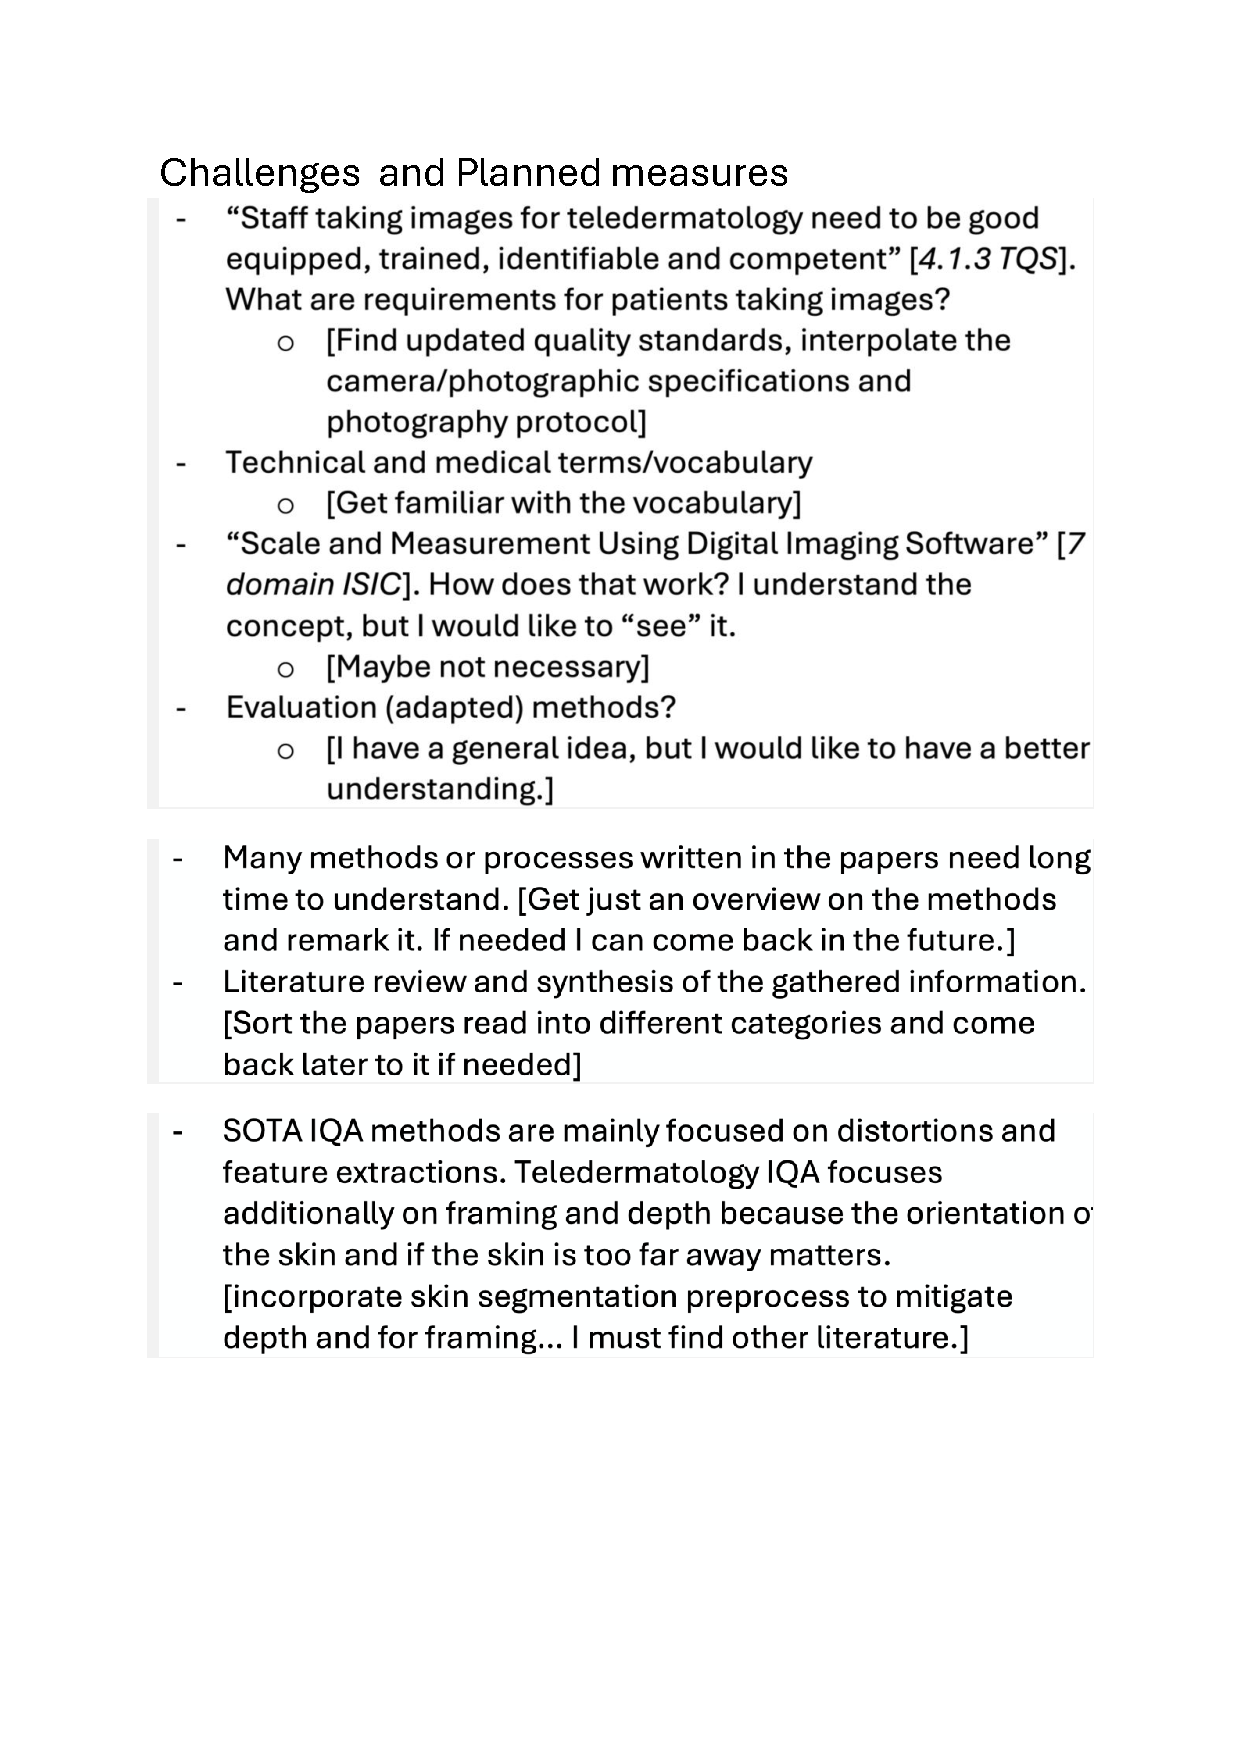
\includepdf[pages=-]{challenges.pdf}
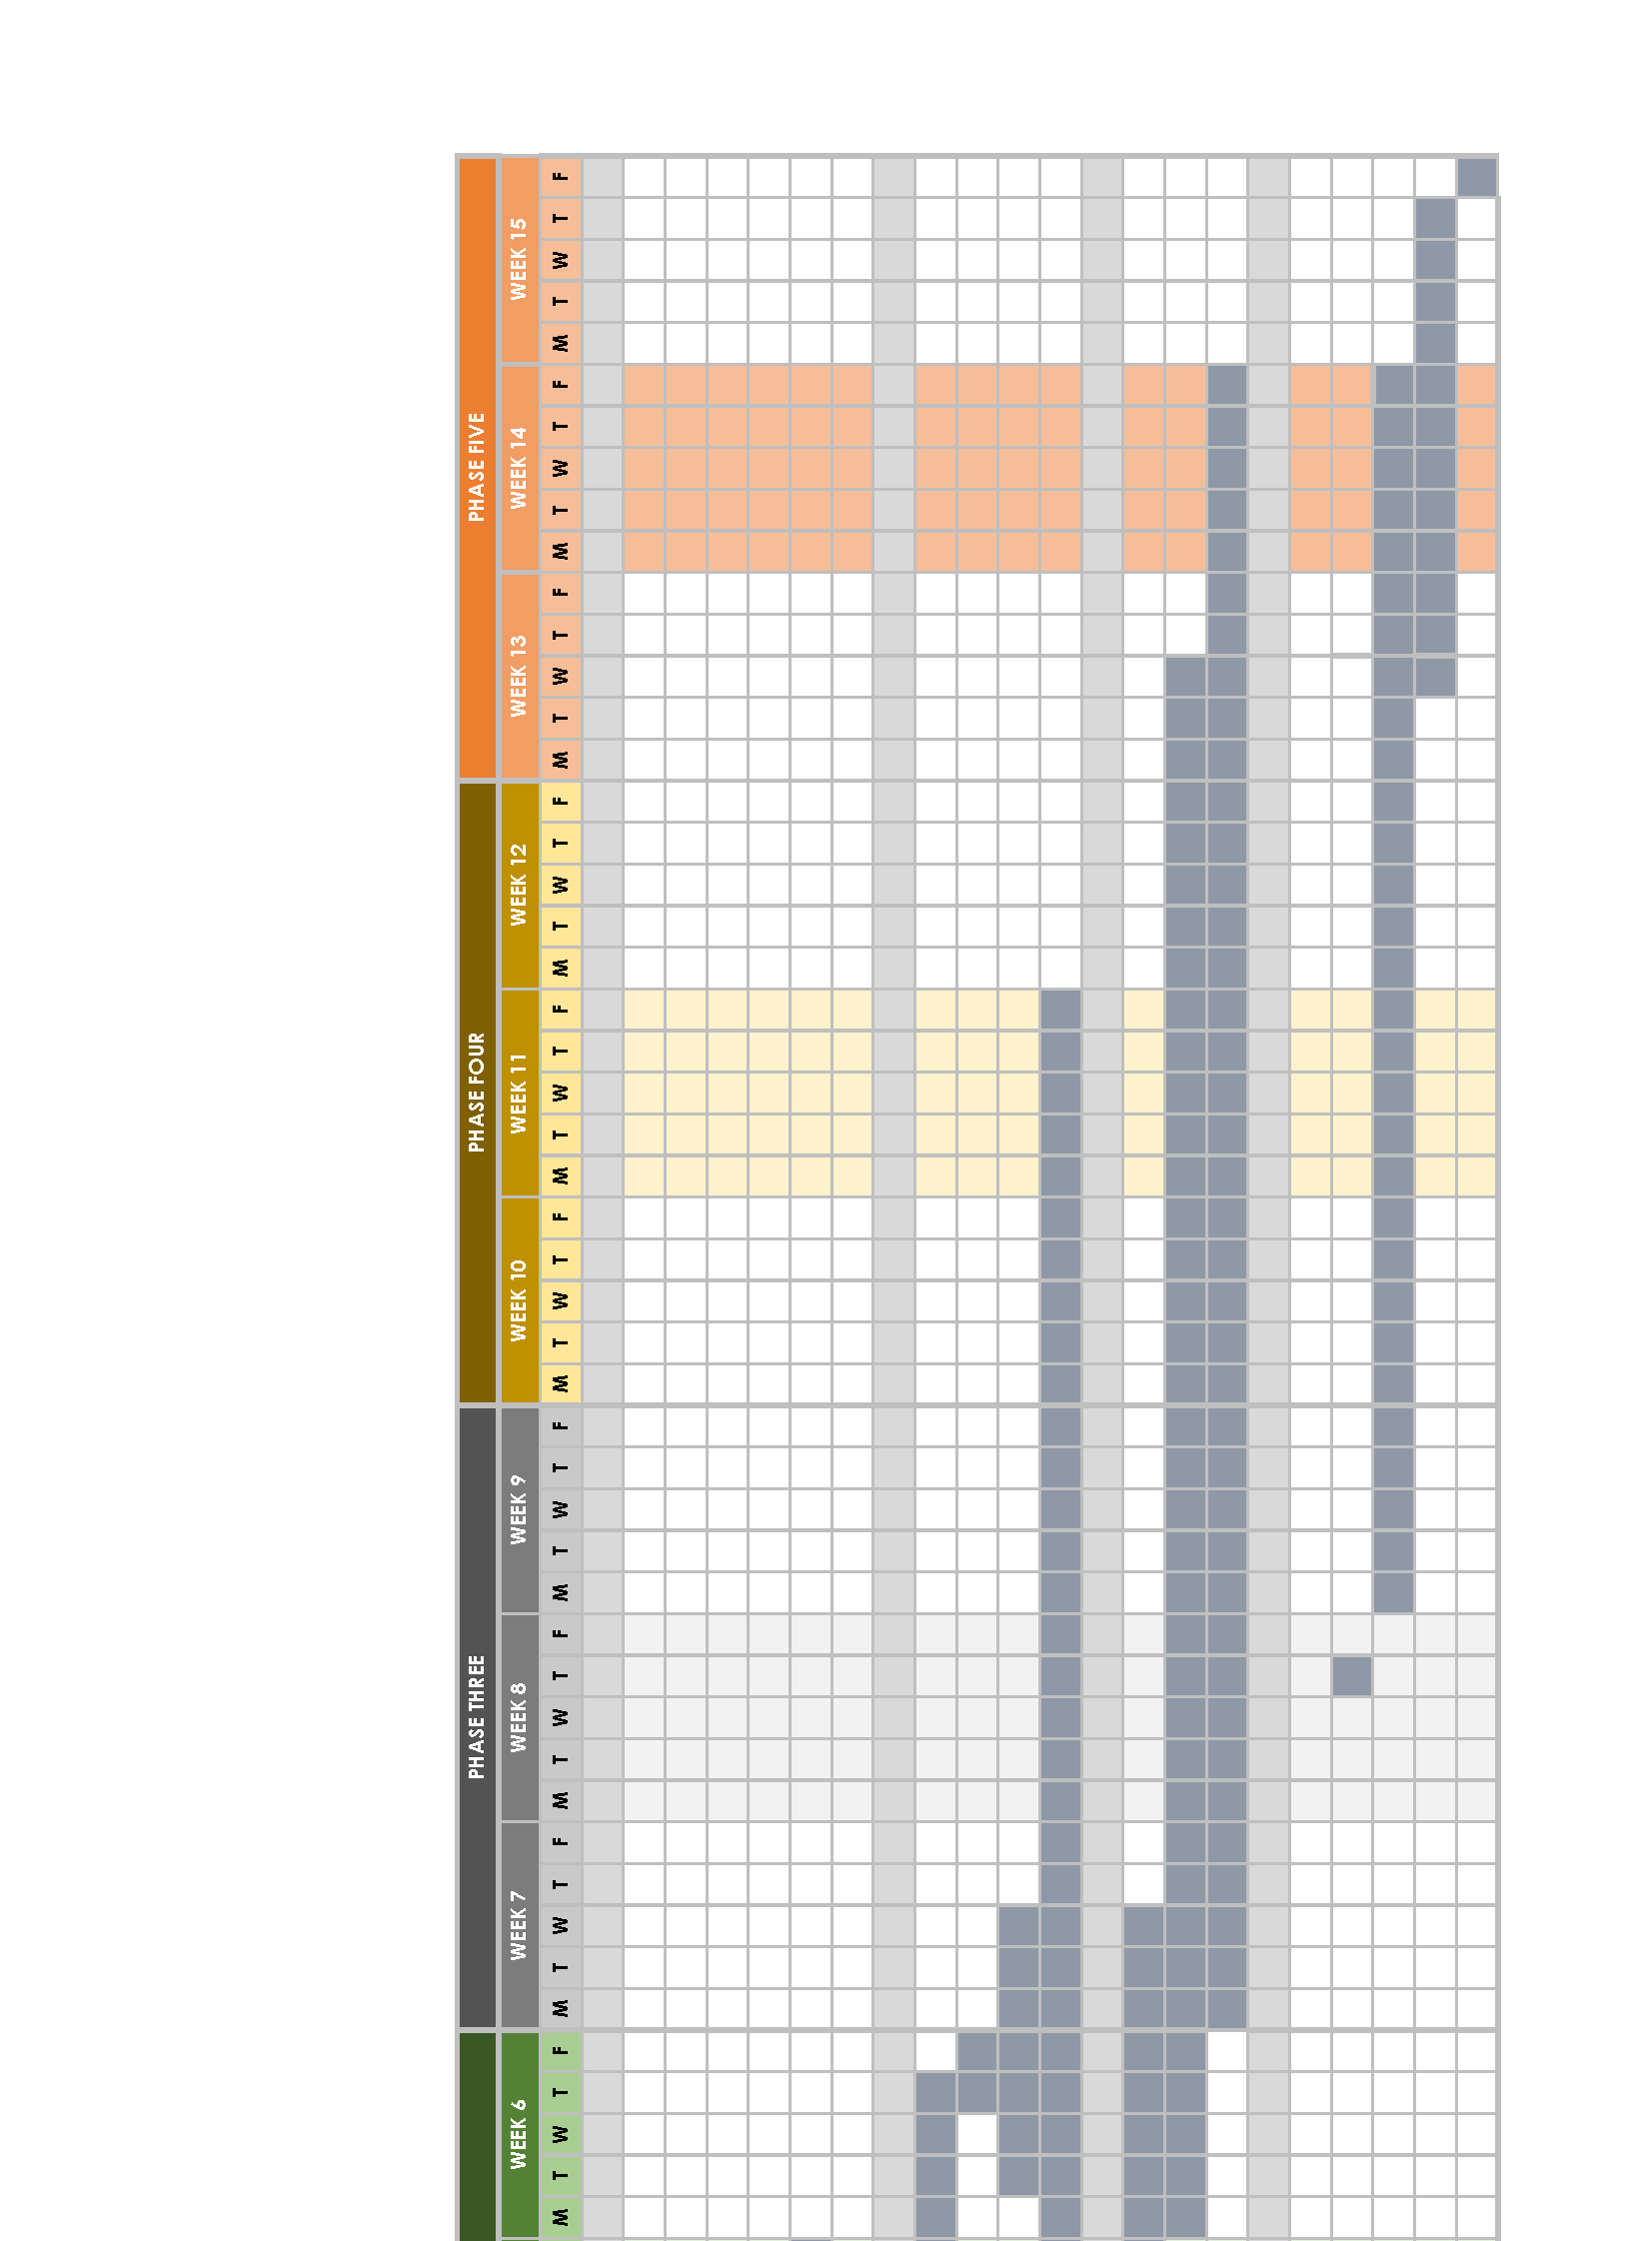
\includepdf[pages=-]{Gantt_BAA.pdf}

\section{Dataset}
\label{sec:Dataset}
Detailed information on image quality assessment (IQA) databases: \par
\begin{itemize}
    \item \textbf{LIVE} (Laboratory for Image \& Video Engineering) dataset \autocite{LIVE} includes 29 reference images and 779 manually distorted images corrupted by 5 types of distortions: JPEG compression (JPEG), JPEG2000 compression (JP2K), white noise (WN), Gaussian blur (GB), and simulated fast fading Rayleigh channel (FF). Each distortion type contains 5 or 4 distortion levels. Most images are 768 $\times$ 512 pixels in size. Each distorted image in this dataset is associated with a Differential Mean Opinion Score (DMOS), scaled from 0 to 100, where 0 indicates no perceivable distortion. 
    \item \textbf{TID2008} (Tampere image database 2008) dataset \autocite{TID2008} includes 25 reference images and 1700 distorted images corrupted by 17 types of distortions, with 4 levels for each distortion type. All images have a fixed resolution of 512 $\times$ 384. This dataset provides MOS values and their standard deviations, with MOS ranging from 0 to 9, where 9 signifies a distortion-free image.
    \item \textbf{TID2013} (Tampere image database 2013) dataset \autocite{TID2013} is extended from TID2008 \autocite{TID2008} by increasing the number of distortion levels to 5, and the number of distortion types to 24. Therefore, 3000 distorted images are generated from 25 pristine images. The subjective testing and data processing steps are similar to that of TID2008. DMOS values for this dataset were derived from over half a million ratings given by nearly a thousand observers, with values ranging from 0 to 9, where higher values denote poorer image quality.
    \item \textbf{CSIQ} (Categorical subjective image quality (CSIQ) database) \autocite{CSIQ} contains 30 pristine images and 866 distorted images corrupted by JPEG, JP2K, WN, GB, additive pink Gaussian noise, and global contrast decrements, with 5 or 4 levels for each distortion type. The resolution is 512 $\times$ 512. Each image in CSIQ is associated with DMOS values obtained from subjective ratings by 25 testers, with DMOS values scaled from 0 to 1, where higher values indicate worse quality.
    \item \textbf{A57} \autocite{A57} includes 3 pristine images and 54 distorted images corrupted by 6 types of distortions, with 3 levels for each distortion type. All images are in gray scale. The resolution is 512 $\times$ 512.
    \item \textbf{WED} (Waterloo exploration database) \autocite{WED} includes 4744 pristine natural images and 94880 distorted images corrupted by JPEG, JP2K, GB, and WN, with 5 levels for each distortion type. The images have various resolutions. No human opinion score is provided, but the authors introduce several alternative test criteria to evaluate the IQA models.
\end{itemize}

\textbf{Multiple Distortions IQA Databases}
\begin{itemize}
    \item \textbf{LIVEMD} (LIVE multiply distorted) \autocite{LIVEMD} database consists of 15 reference images and 405 multiply distorted images. The database includes one/double-fold artifacts. Each multiply distorted image is corrupted under two multiple distortion scenarios: Gaussian blur followed by JPEG and Gaussian blur followed by white noise. All images have a resolution of 1280 $\times$ 720. DMOS values for each distorted image range from 0 to 100.
    \item \textbf{Multiply distorted image database 2013 (MDID2013)} \autocite{MDID2013}: MDID2013 has a total of 12 pristine images and 324 distorted images. Each pristine image is corrupted successively by Gaussian blur, white noise, and JPEG. The images have resolutions of 768 $\times$ 512 or 1280 $\times$ 720.
    \item \textbf{Multiply distorted image database 2016 (MDID2016)} \autocite{MDID2016}: MDID2016 consists of 20 reference images and 1600 distorted images. Five distortion types are introduced, i.e., white noise, Gaussian blur, JPEG, JPEG2000, and contrast change (CC). The order of distortions is as follows: Gaussian blur or CC first, JPEG or JPEG2000 second, and white noise last. All distorted images are with random types and levels of distortions. The image resolution is 512 $\times$ 384.
\end{itemize}

\textbf{Screen Content IQA Databases}
\begin{itemize}
    \item \textbf{Screen Image Quality Assessment Database (SIQAD)} \autocite{SIQAD}: SIQAD includes 20 pristine and 980 distorted screen content images (SCIs). Distortion types include white noise (WN), Gaussian blur (GB), color cast (CC), JPEG, JPEG2000 (JP2K), motion blur (MB), and layer segmentation-based compression, with 7 levels for each type. The images have various resolutions near 700 $\times$ 700.
    \item \textbf{Screen Content Image Quality (SCIQ) Database} \autocite{SCIQ}: SCIQ consists of 40 pristine and 1800 distorted SCIs corrupted by 9 types of distortions, including WN, GB, MB, CC, JPEG, JP2K, color saturation change (CSC), color quantization with dithering (CQD), and the screen content coding extension of High Efficiency Video Coding (HEVC-SCC). Five distortion levels are considered. The resolution is fixed at 1280 $\times$ 720.
    \item \textbf{Cross-Content-Type (CCT) Database} \autocite{CCT}: CCT is constructed to conduct cross-content-type IQA research. CCT consists of 72 pristine and 1320 distorted natural scene images (NSIs), computer graphic images (CGIs), and SCIs. Two distortion types are considered, i.e., HEVC and HEVC-SCC coding, with 11 distortion levels for each type. The image resolution is either 1920 $\times$ 1080 or 1280 $\times$ 720.
    \item \textbf{Hybrid Screen Content and Natural Scene Image Database (HSNID)} \autocite{HSNID}: HSNID has 10 pristine NSIs and 10 pristine SCIs, and 600 distorted NSIs and SCIs corrupted by WN, GB, MB, CC, JPEG, and JP2K, with 5 distortion levels for each type.
\end{itemize}

\textbf{Authentic Distortions IQA Databases}
\begin{itemize}
    \item \textbf{LIVE in the wild image quality challenge database} \autocite{LIVE_Wild} includes 1162 authentically distorted images captured using a variety of mobile devices. Complex real distortions, which are not well-modeled by the synthetic distortions are included. All images are cropped to the resolution of 500 $\times$ 500. A novel crowdsourcing system was employed to gather over 350,000 opinion scores from 8100 observers, ensuring the objectivity of the MOS values obtained.
    \item \textbf{Camera image database (CID2013)} \autocite{CID2013}: CID2013 is designed to test no-reference IQA algorithms. It includes 480 real images captured from 8 typical scenes using 79 consumer cameras and mobile phones. The images are rated from 5 aspects: the overall quality, sharpness, graininess, lightness, and color saturation scales. The images are scaled to a size of 1600 $\times$ 1200.
\end{itemize}

\clearpage
\section{Degradation Types}
\label{sec:Degradation_Types}
The dataset used in this thesis is augmented with synthetic degradations. The following figures below show the different levels of intensity for the degradations of each distortion group. \par
\begin{figure*}[ht]
    \centering
    \setlength{\tabcolsep}{1pt}
    \Large
    \resizebox{\textwidth}{!}{%
        \begin{tabular}{C{5em}ccccc}
            & Level 1 & Level 2 & Level 3 & Level 4 & Level 5 \\
            Brighten & 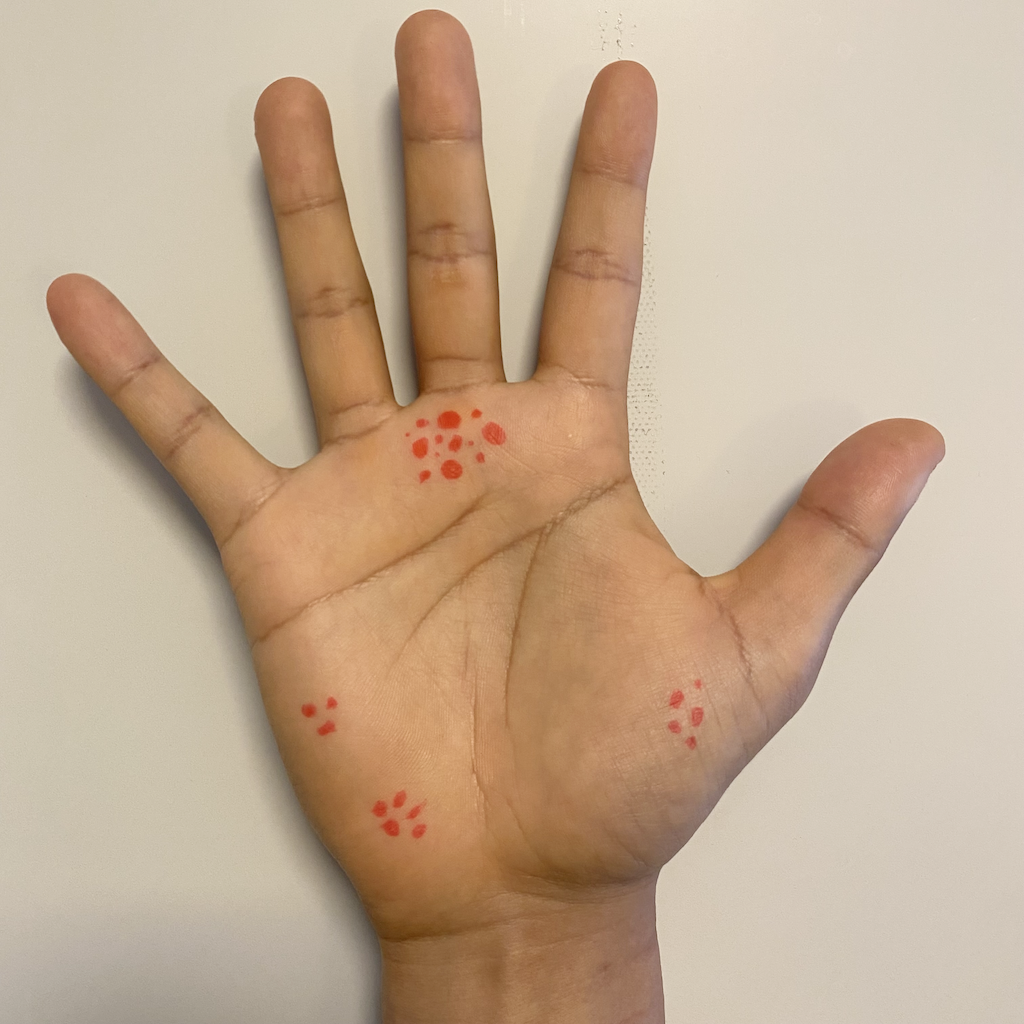
\includegraphics[width=\gridimagewidth,valign=m]{img/supplementary/lighting/brighten/0_brighten_0.0.png} & 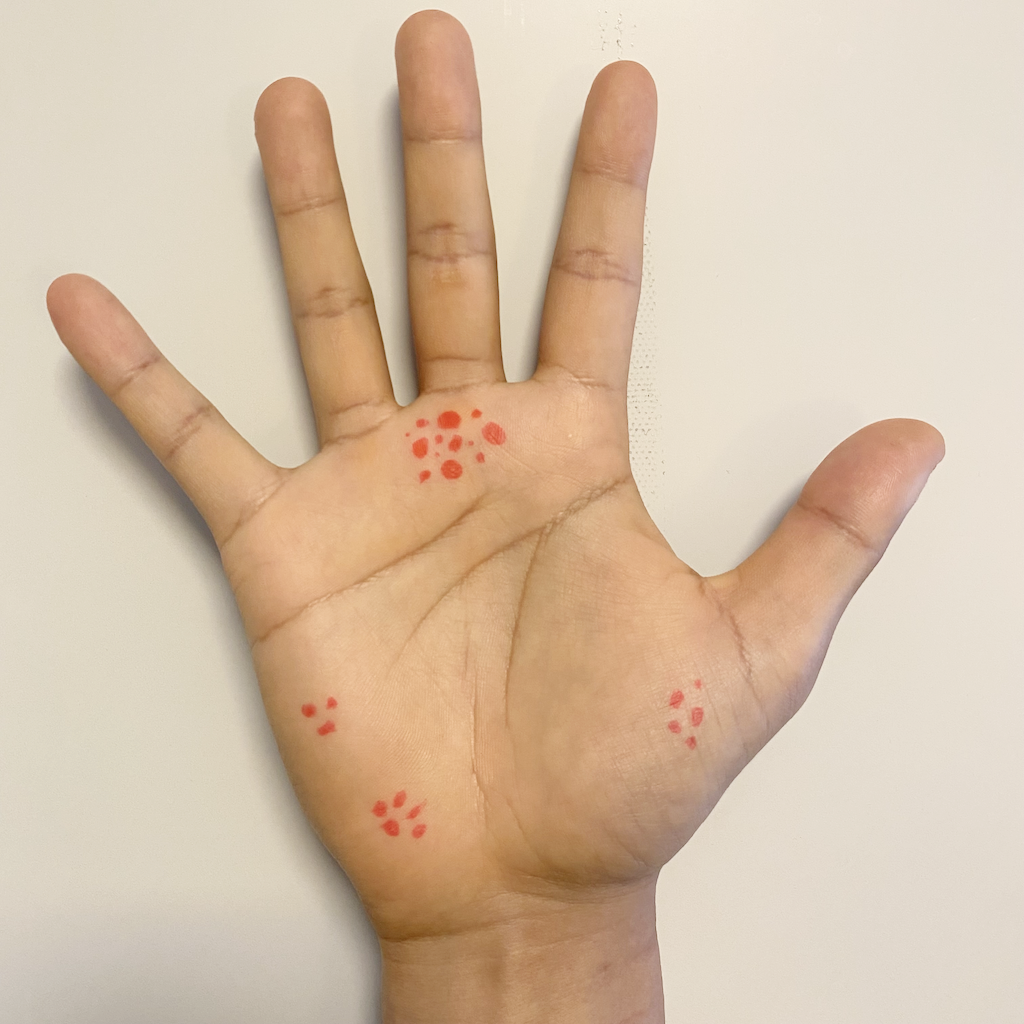
\includegraphics[width=\gridimagewidth,valign=m]{img/supplementary/lighting/brighten/0_brighten_0.2.png} & 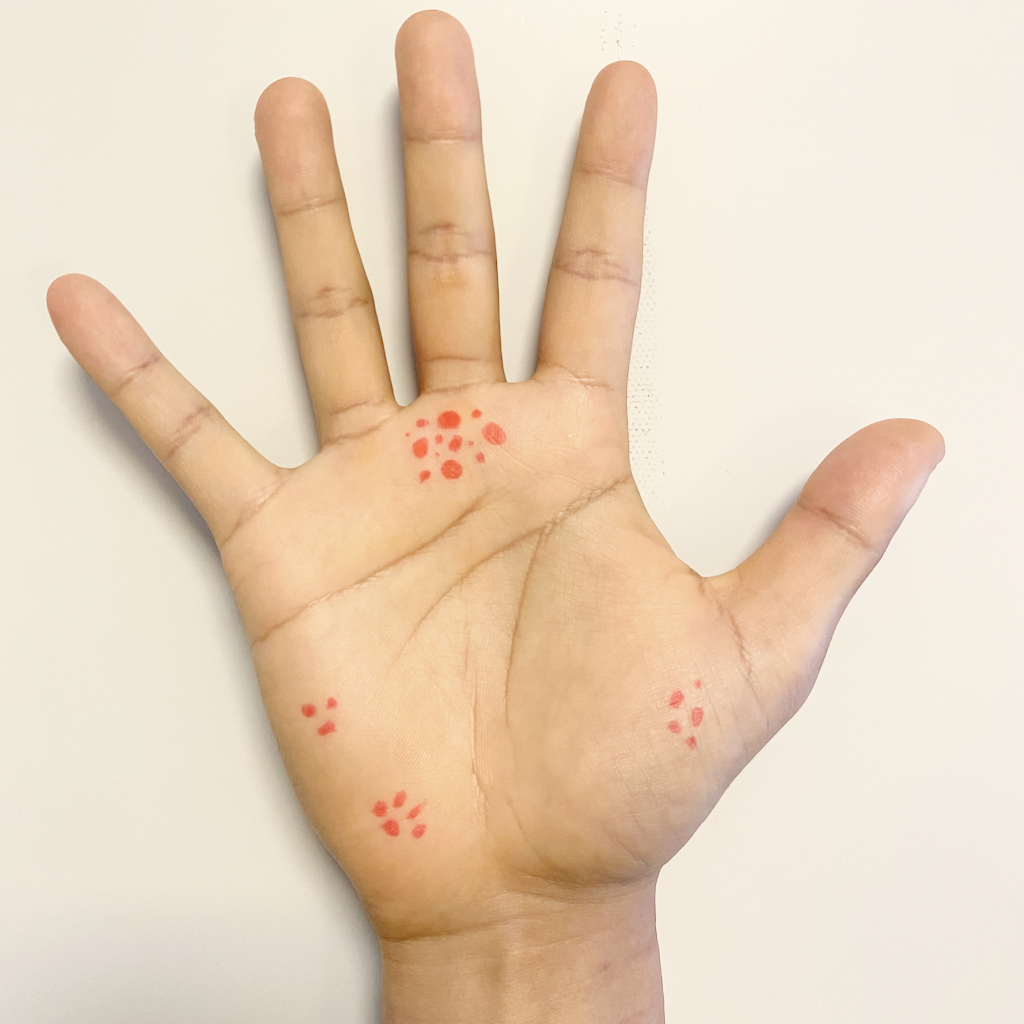
\includegraphics[width=\gridimagewidth,valign=m]{img/supplementary/lighting/brighten/0_brighten_0.4.png} & 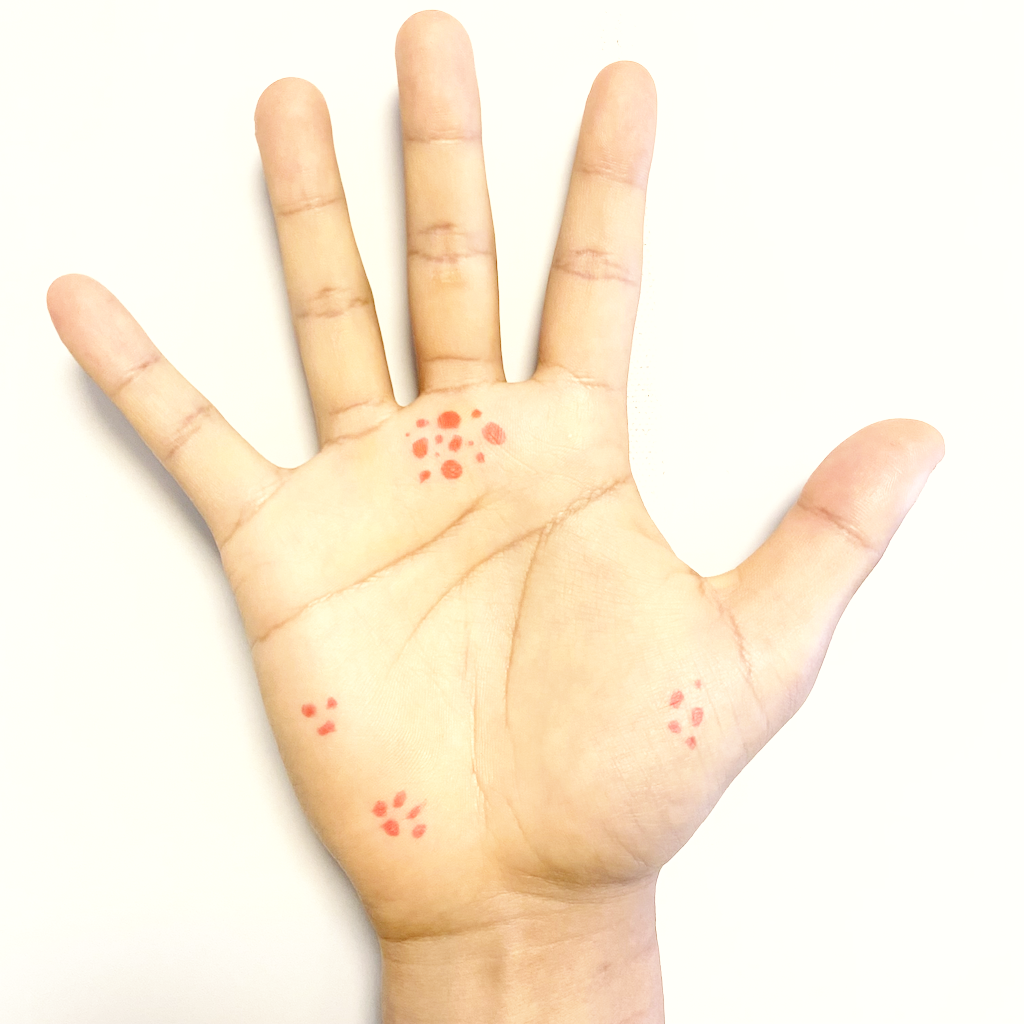
\includegraphics[width=\gridimagewidth,valign=m]{img/supplementary/lighting/brighten/0_brighten_0.7.png} & 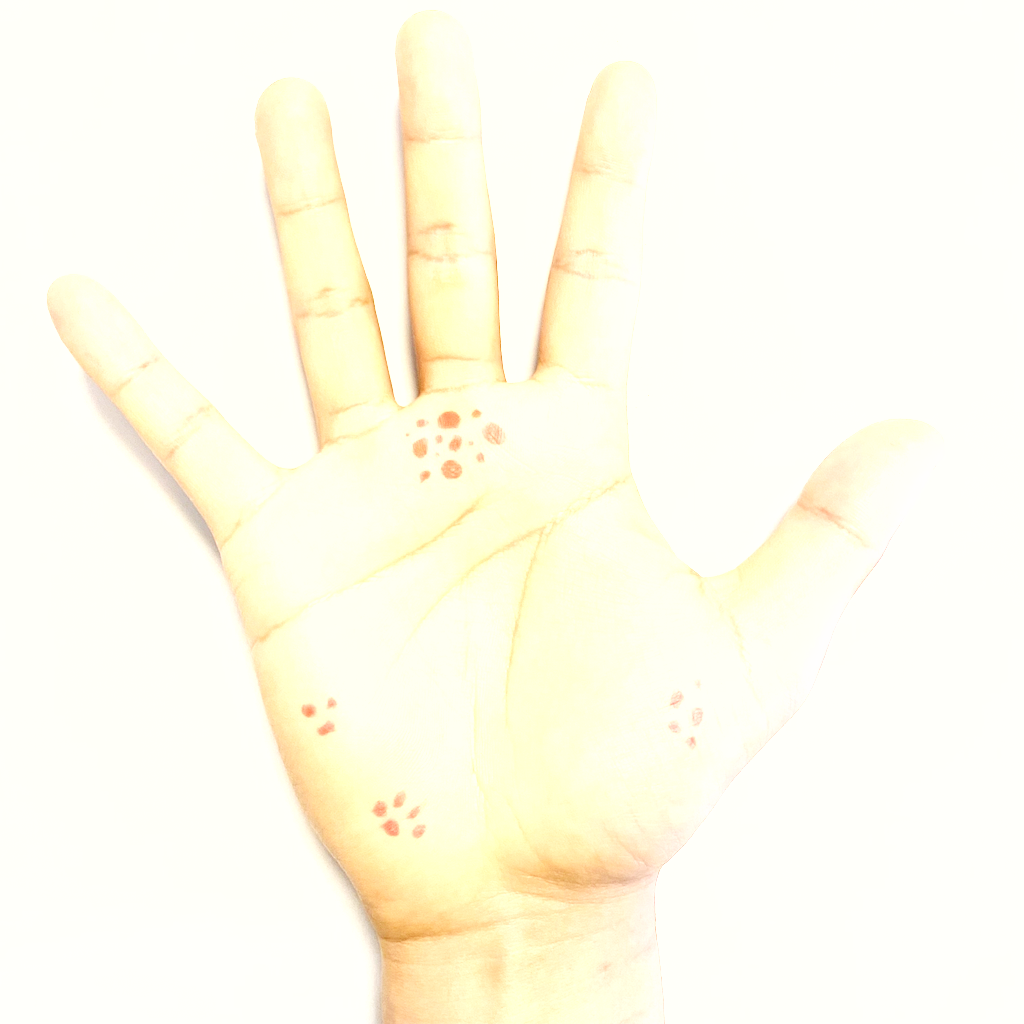
\includegraphics[width=\gridimagewidth,valign=m]{img/supplementary/lighting/brighten/0_brighten_1.1.png} \\ [6.15ex]
            Darken & 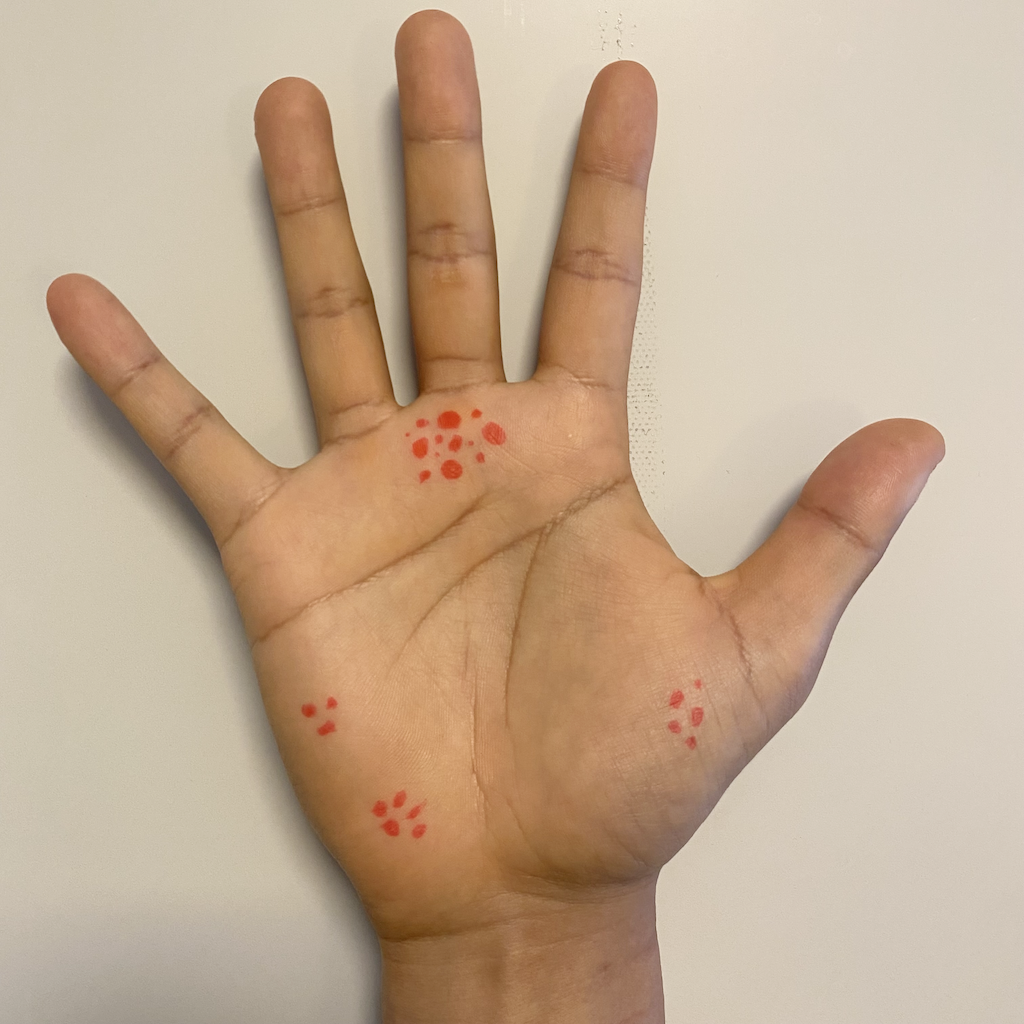
\includegraphics[width=\gridimagewidth,valign=m]{img/supplementary/lighting/darken/0_darken_0.0.png} & 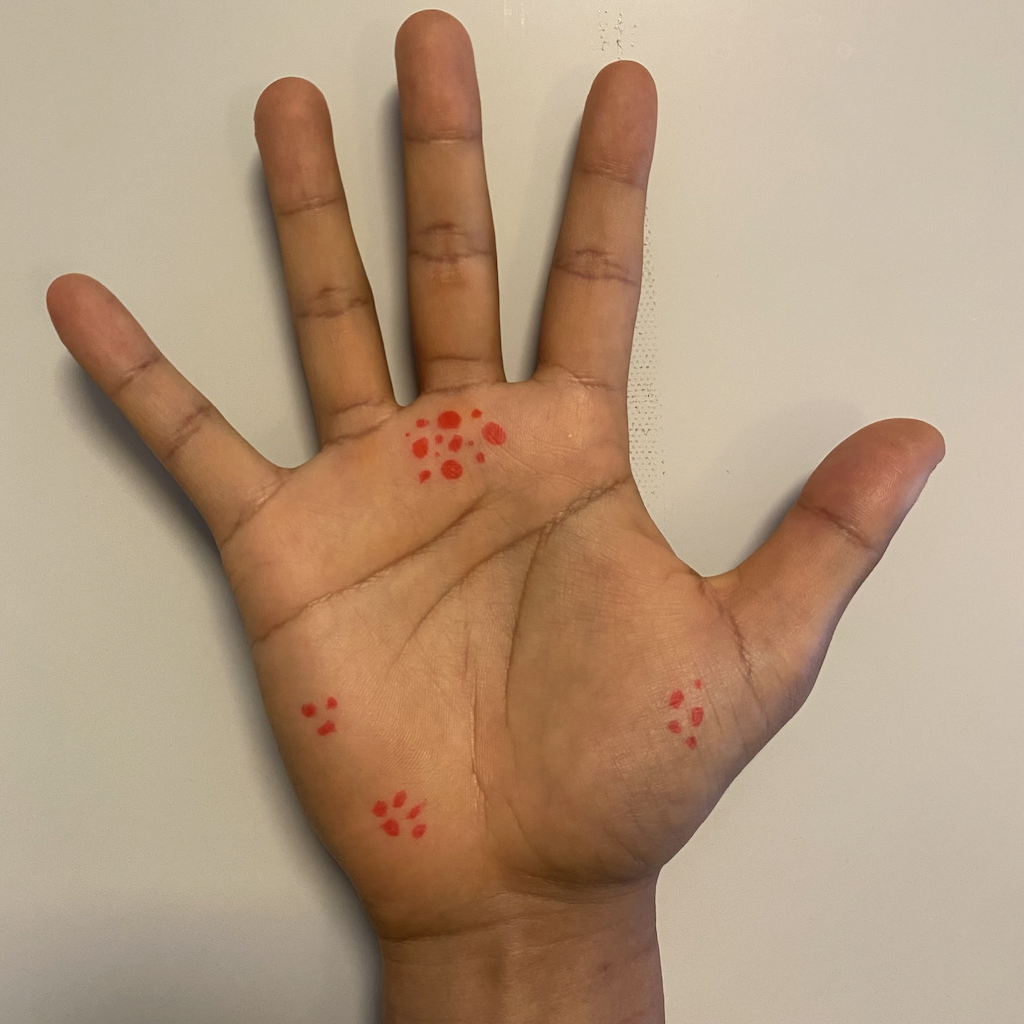
\includegraphics[width=\gridimagewidth,valign=m]{img/supplementary/lighting/darken/0_darken_0.2.png} & 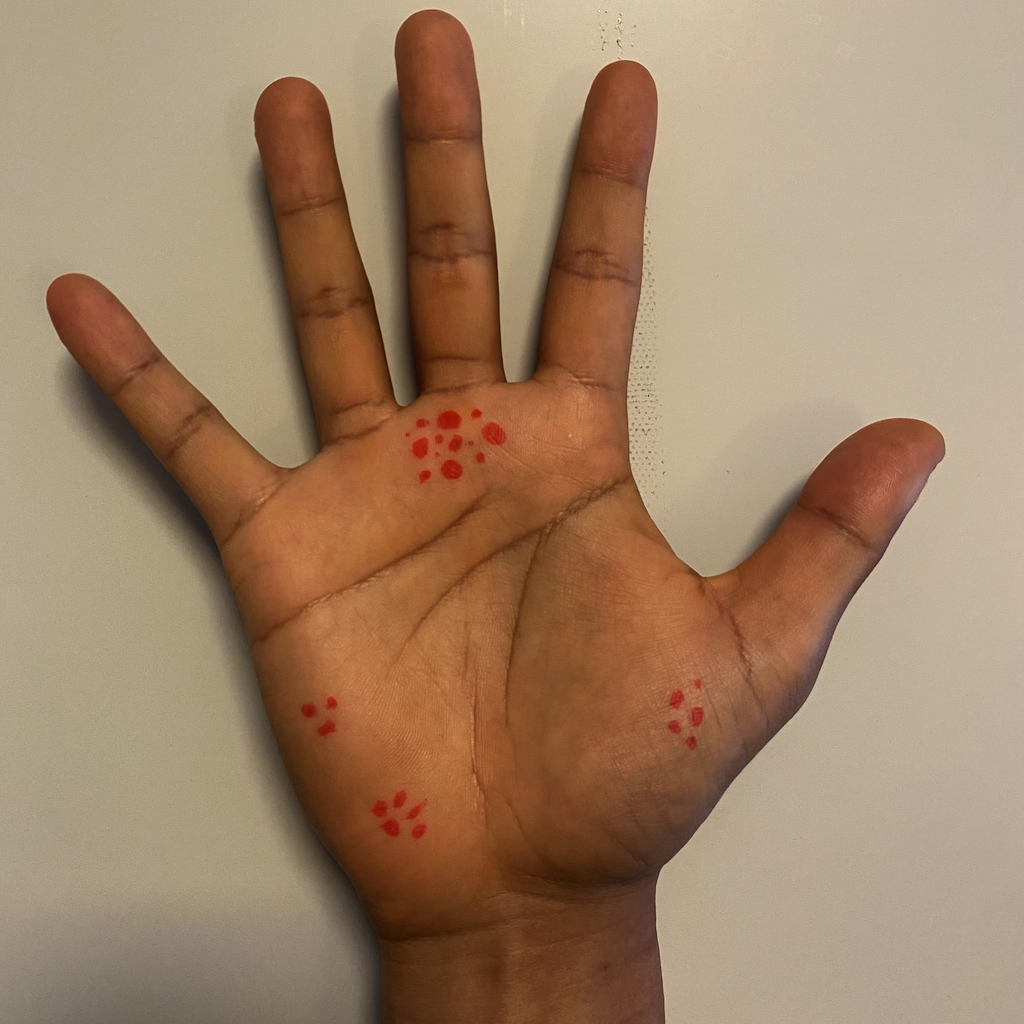
\includegraphics[width=\gridimagewidth,valign=m]{img/supplementary/lighting/darken/0_darken_0.4.png} & 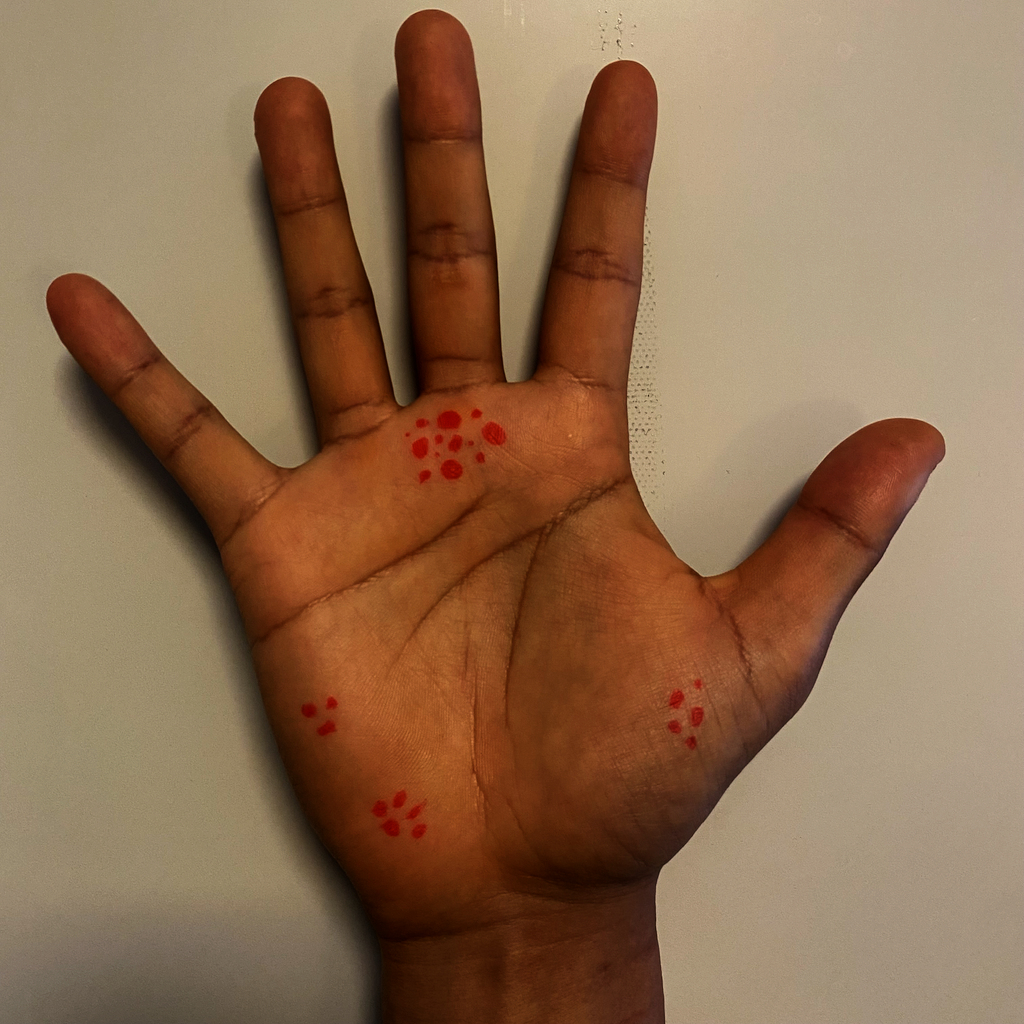
\includegraphics[width=\gridimagewidth,valign=m]{img/supplementary/lighting/darken/0_darken_0.6.png} & 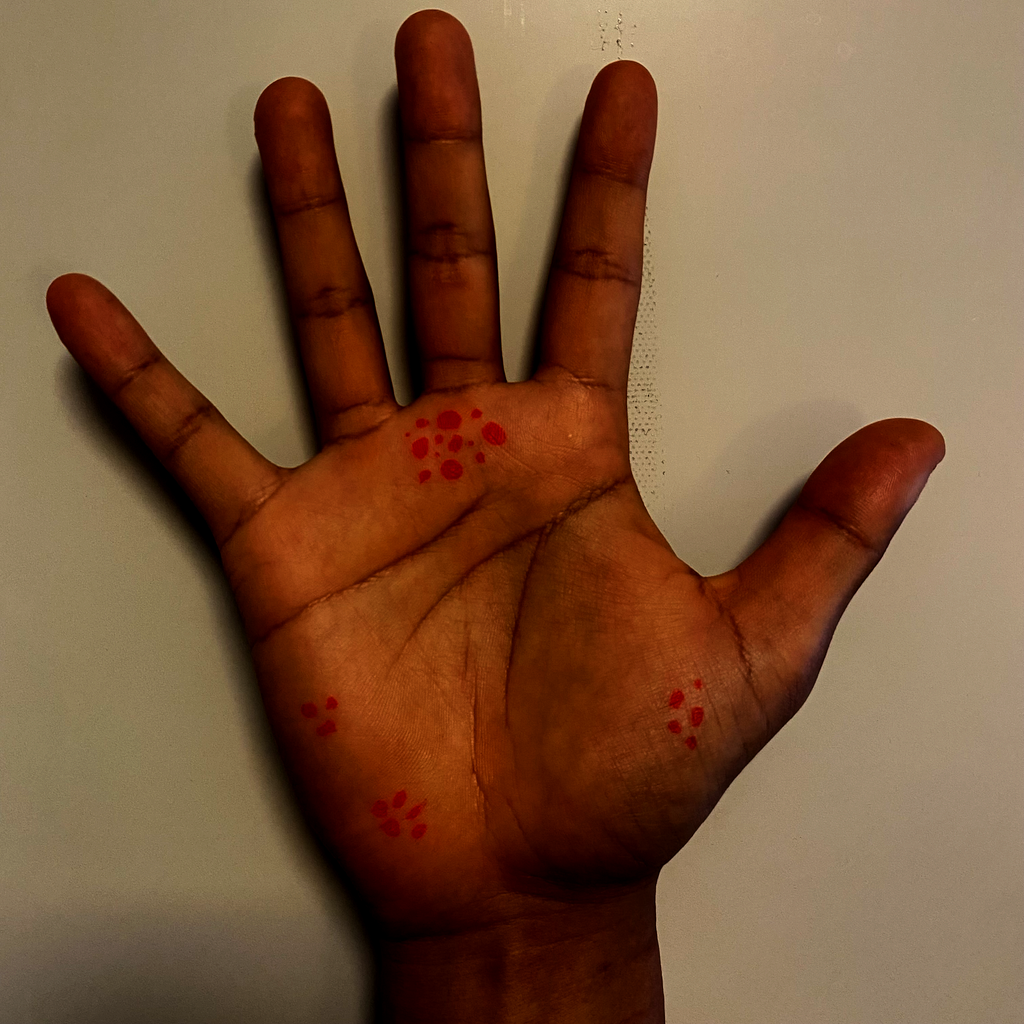
\includegraphics[width=\gridimagewidth,valign=m]{img/supplementary/lighting/darken/0_darken_0.8.png} \\ [6.15ex]
        \end{tabular}
    }
    \caption{Visualization of the degradation types belonging to the \textit{Brightness change} group for increasing levels of intensity.}
    \label{fig:brightness_change_supplementary}
\end{figure*}

\begin{figure*}[ht]
    \centering
    \setlength{\tabcolsep}{1pt}
    \Large
    \resizebox{\textwidth}{!}{%
        \begin{tabular}{C{5em}ccccc}
            & Level 1 & Level 2 & Level 3 & Level 4 & Level 5 \\
            Color block & 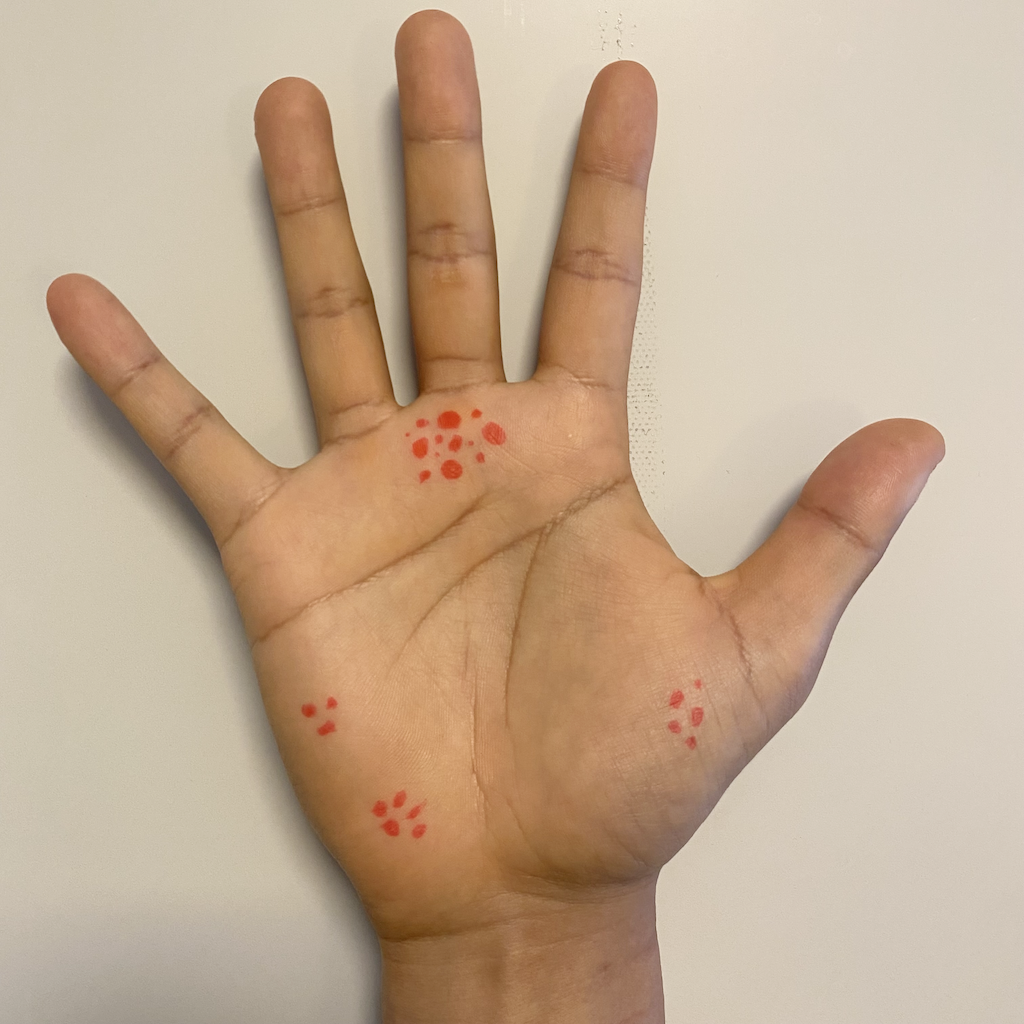
\includegraphics[width=\gridimagewidth,valign=m]{img/supplementary/background/color_block/0_color_block_0.0.png} & 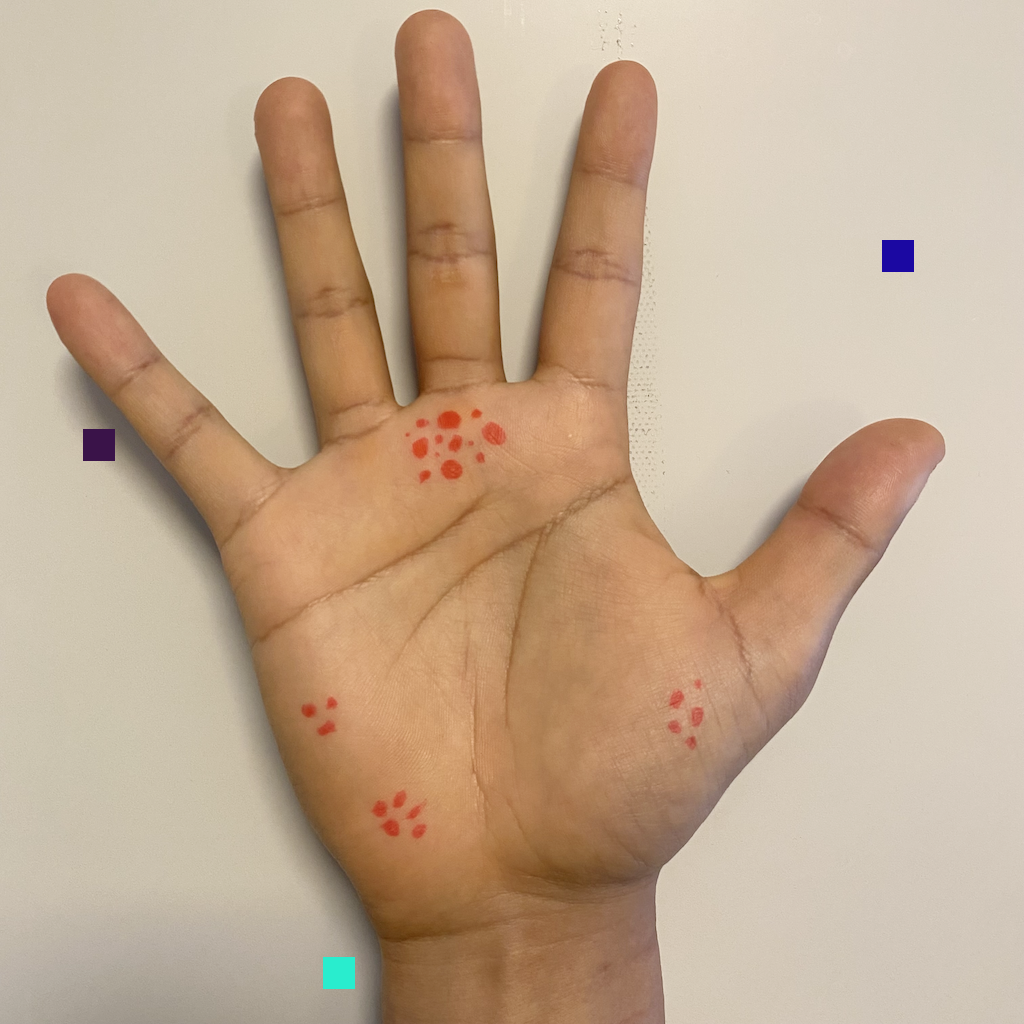
\includegraphics[width=\gridimagewidth,valign=m]{img/supplementary/background/color_block/0_color_block_0.5.png} & 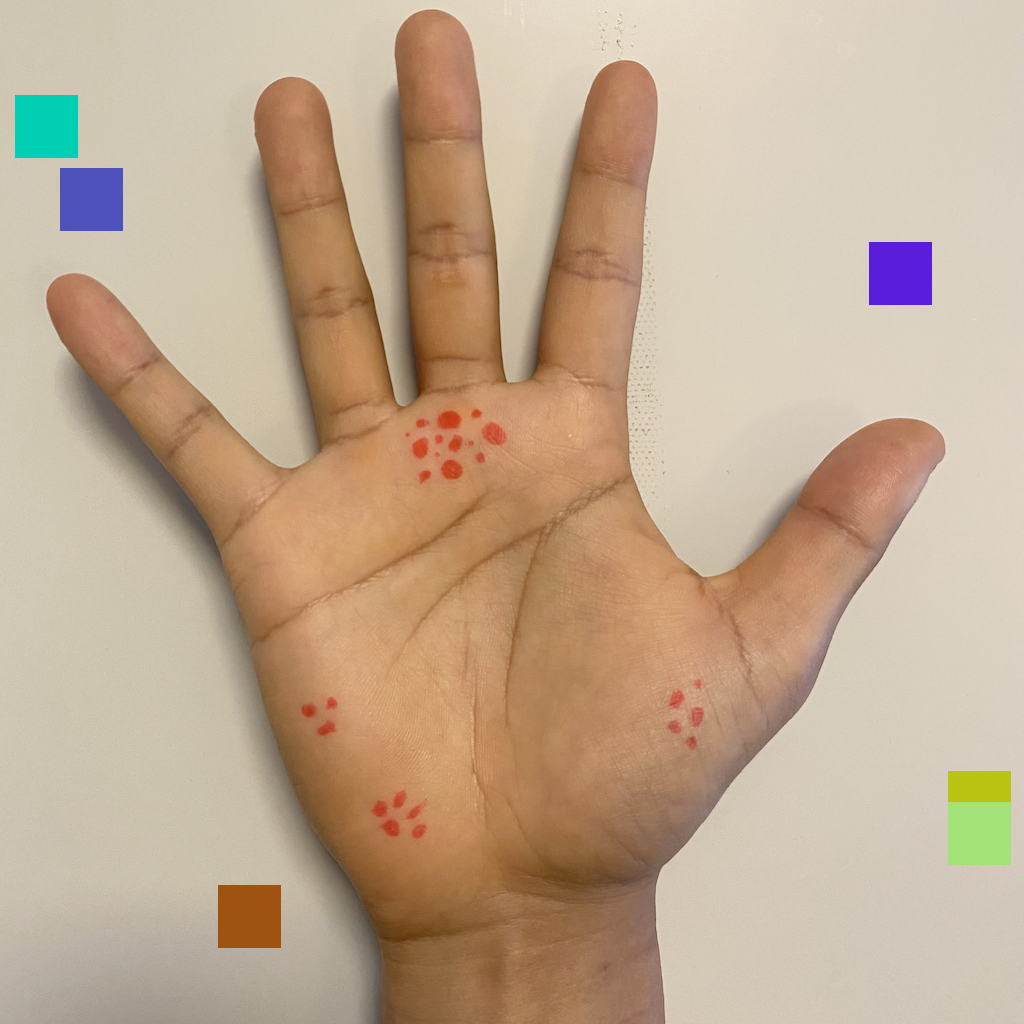
\includegraphics[width=\gridimagewidth,valign=m]{img/supplementary/background/color_block/0_color_block_1.0.png} & 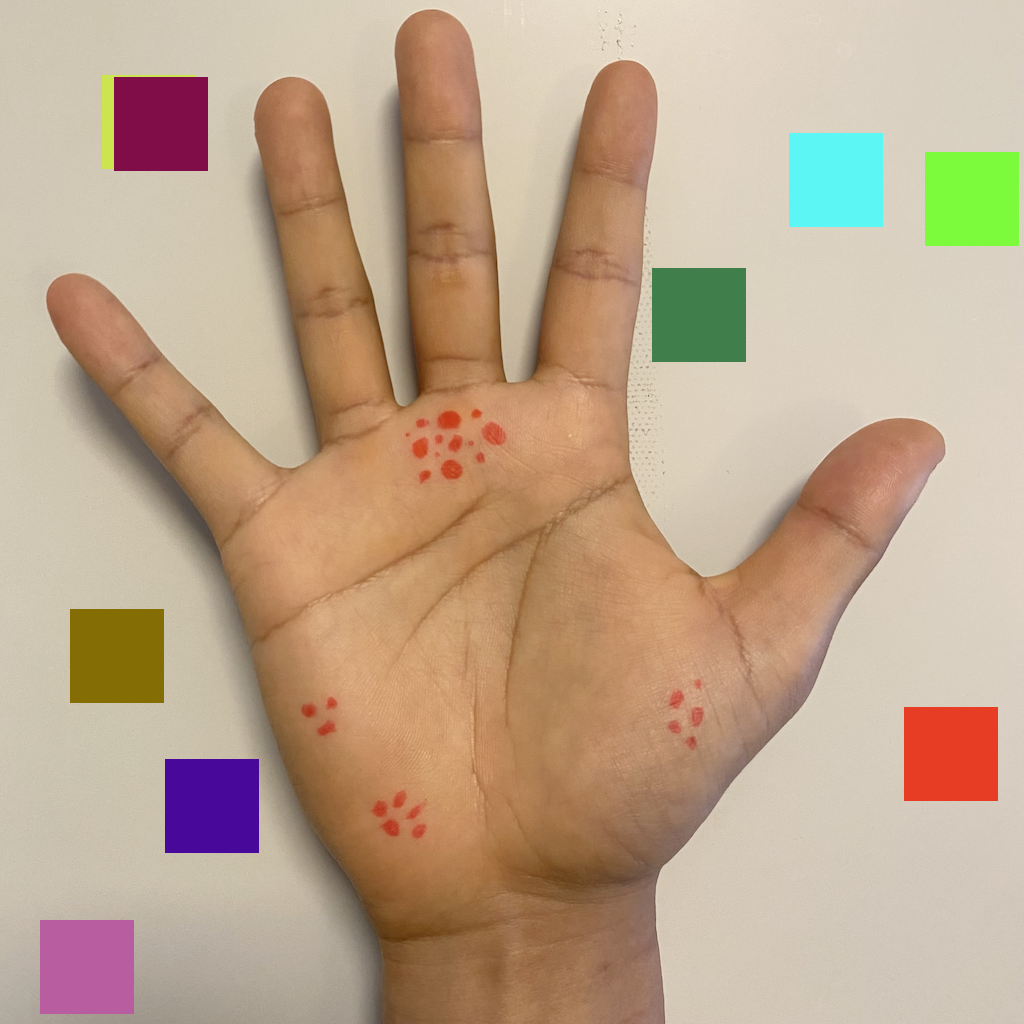
\includegraphics[width=\gridimagewidth,valign=m]{img/supplementary/background/color_block/0_color_block_1.5.png} & 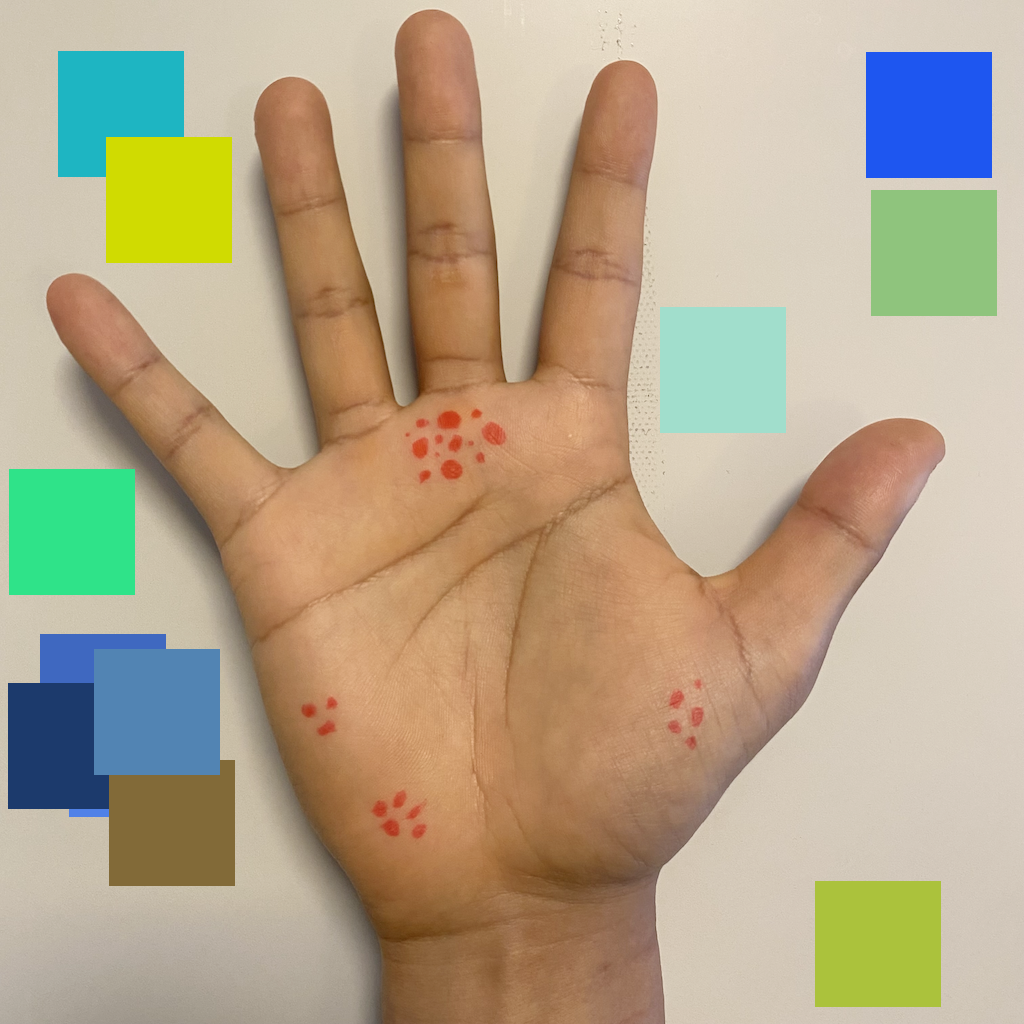
\includegraphics[width=\gridimagewidth,valign=m]{img/supplementary/background/color_block/0_color_block_2.0.png} \\ [6.15ex]
        \end{tabular}
    }
    \caption{Visualization of the degradation types belonging to the \textit{Background color} group for increasing levels of intensity.}
    \label{fig:background_supplementary}
\end{figure*}

\begin{figure*}[ht]
    \centering
    \setlength{\tabcolsep}{1pt}
    \Large
    \resizebox{\textwidth}{!}{%
        \begin{tabular}{C{5em}ccccc}
            & Level 1 & Level 2 & Level 3 & Level 4 & Level 5 \\
            Field of view & 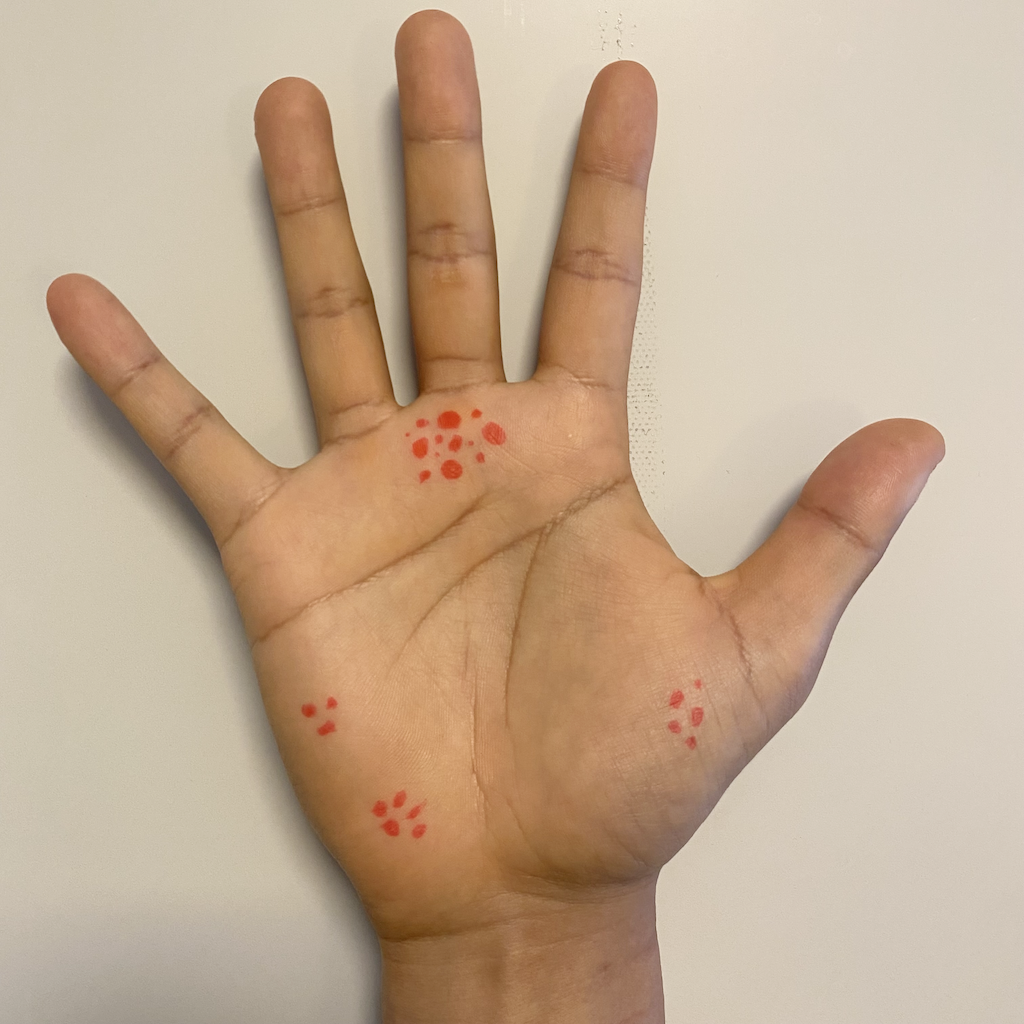
\includegraphics[width=\gridimagewidth,valign=m]{img/supplementary/field_of_view/crop_image/0_crop_image_0.png} & 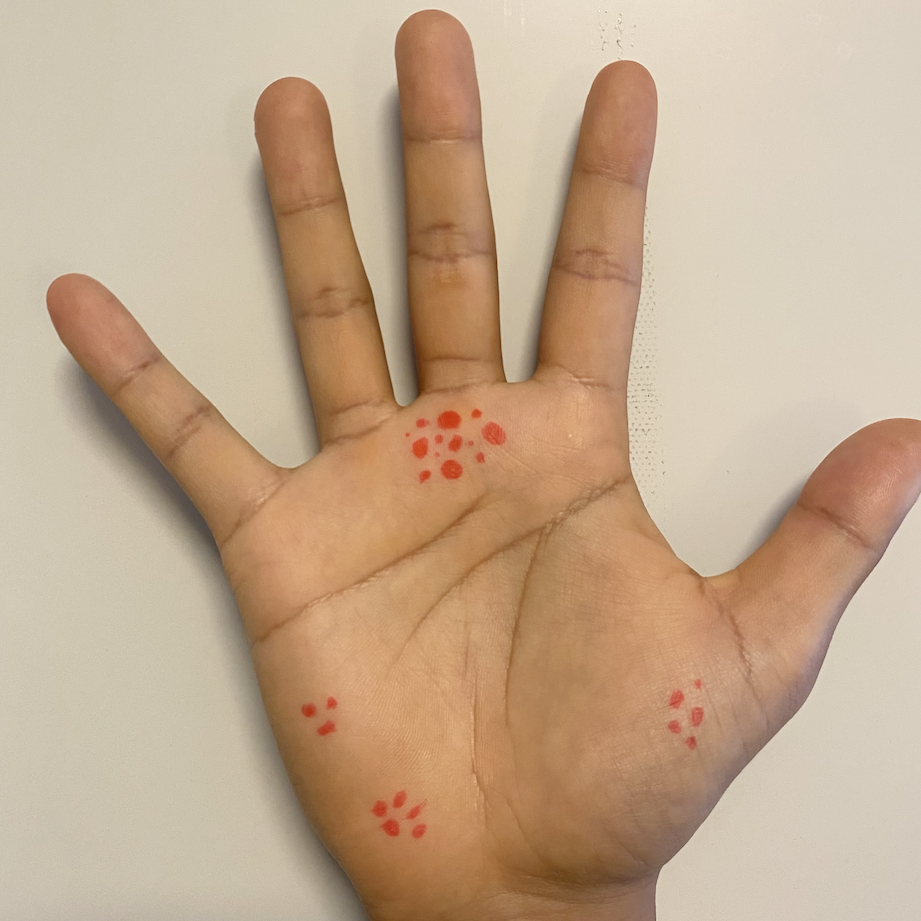
\includegraphics[width=\gridimagewidth,valign=m]{img/supplementary/field_of_view/crop_image/0_crop_image_1.png} & 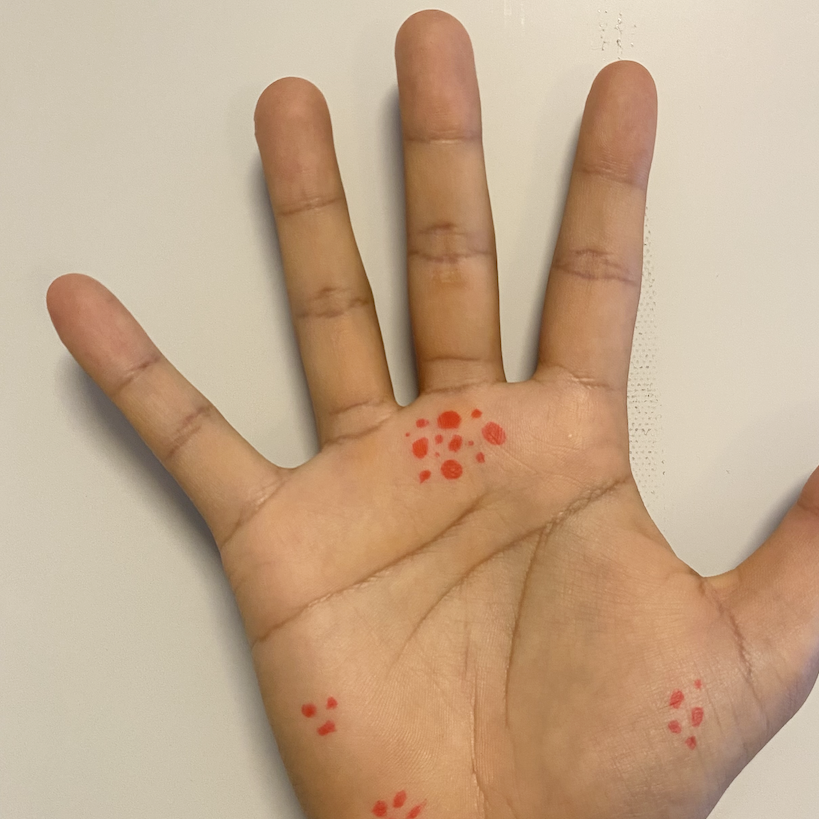
\includegraphics[width=\gridimagewidth,valign=m]{img/supplementary/field_of_view/crop_image/0_crop_image_2.png} & 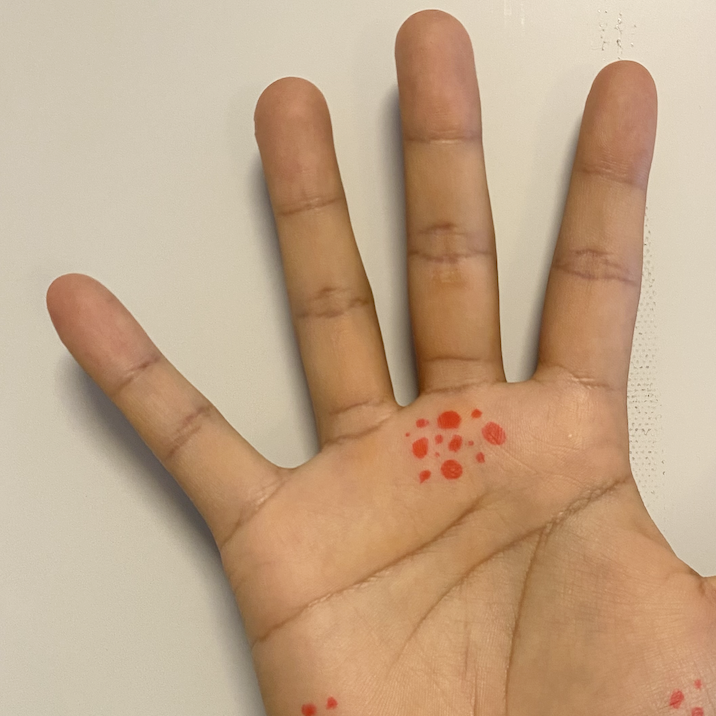
\includegraphics[width=\gridimagewidth,valign=m]{img/supplementary/field_of_view/crop_image/0_crop_image_3.png} & 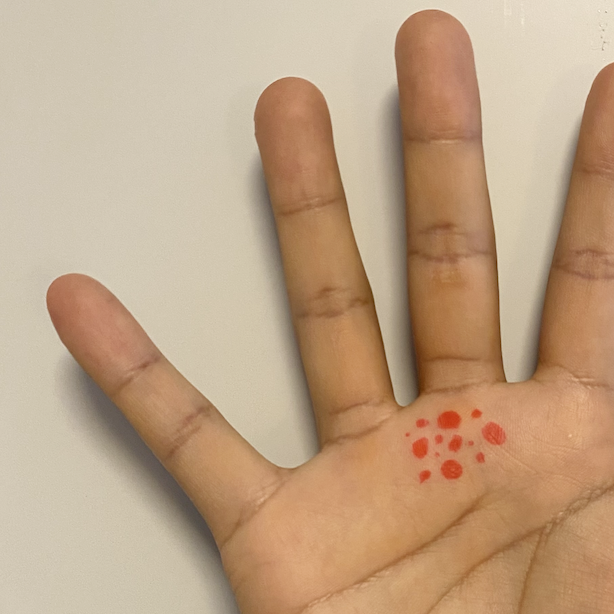
\includegraphics[width=\gridimagewidth,valign=m]{img/supplementary/field_of_view/crop_image/0_crop_image_4.png} \\ [6.15ex]
        \end{tabular}
    }
    \caption{Visualization of the degradation types belonging to the \textit{Field of View} group for increasing levels of intensity.}
    \label{fig:field_of_view_supplementary}
\end{figure*}

\begin{figure*}[ht]
    \centering
    \setlength{\tabcolsep}{1pt}
    \Large
    \resizebox{\textwidth}{!}{%
        \begin{tabular}{C{5em}ccccc}
            & Level 1 & Level 2 & Level 3 & Level 4 & Level 5 \\
            Perspective bottom & 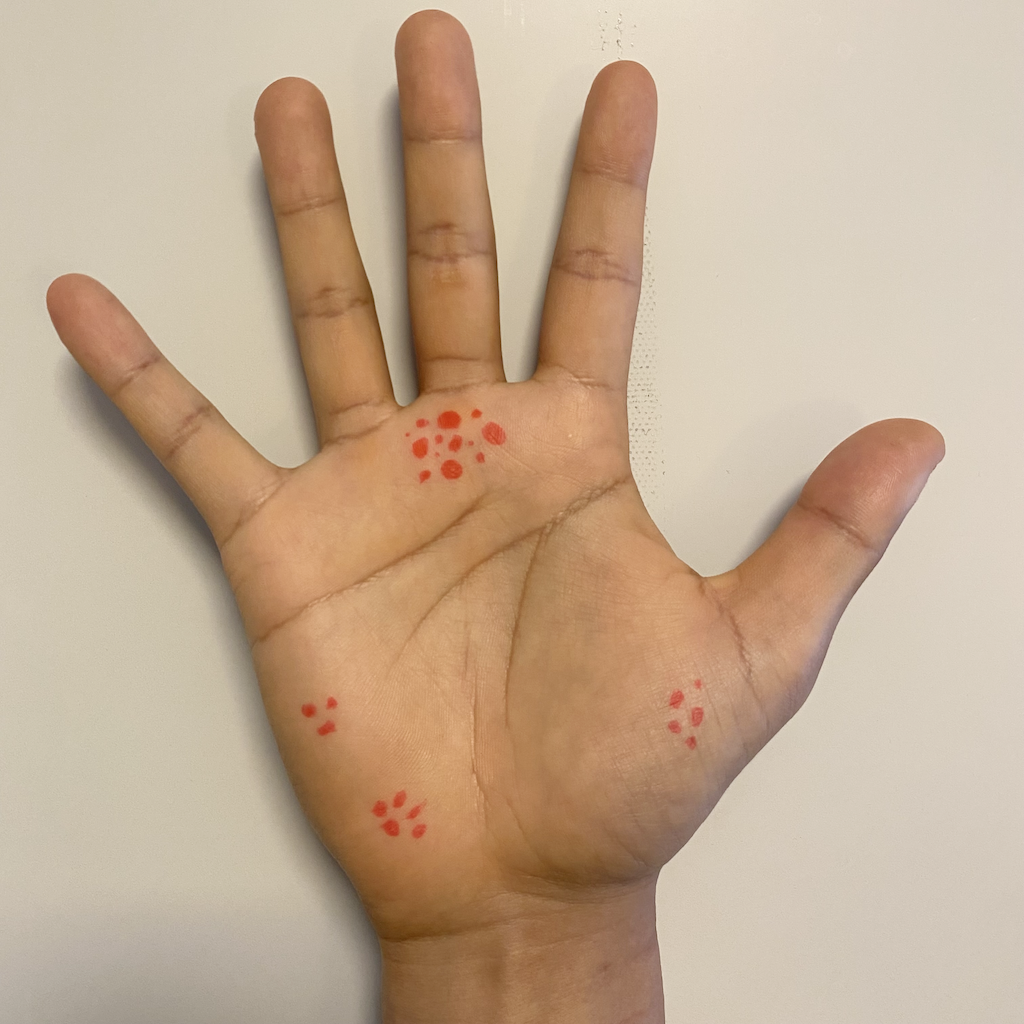
\includegraphics[width=\gridimagewidth,valign=m]{img/supplementary/orientation/perspective_bottom/0_perspective_bottom_0.0.png} & 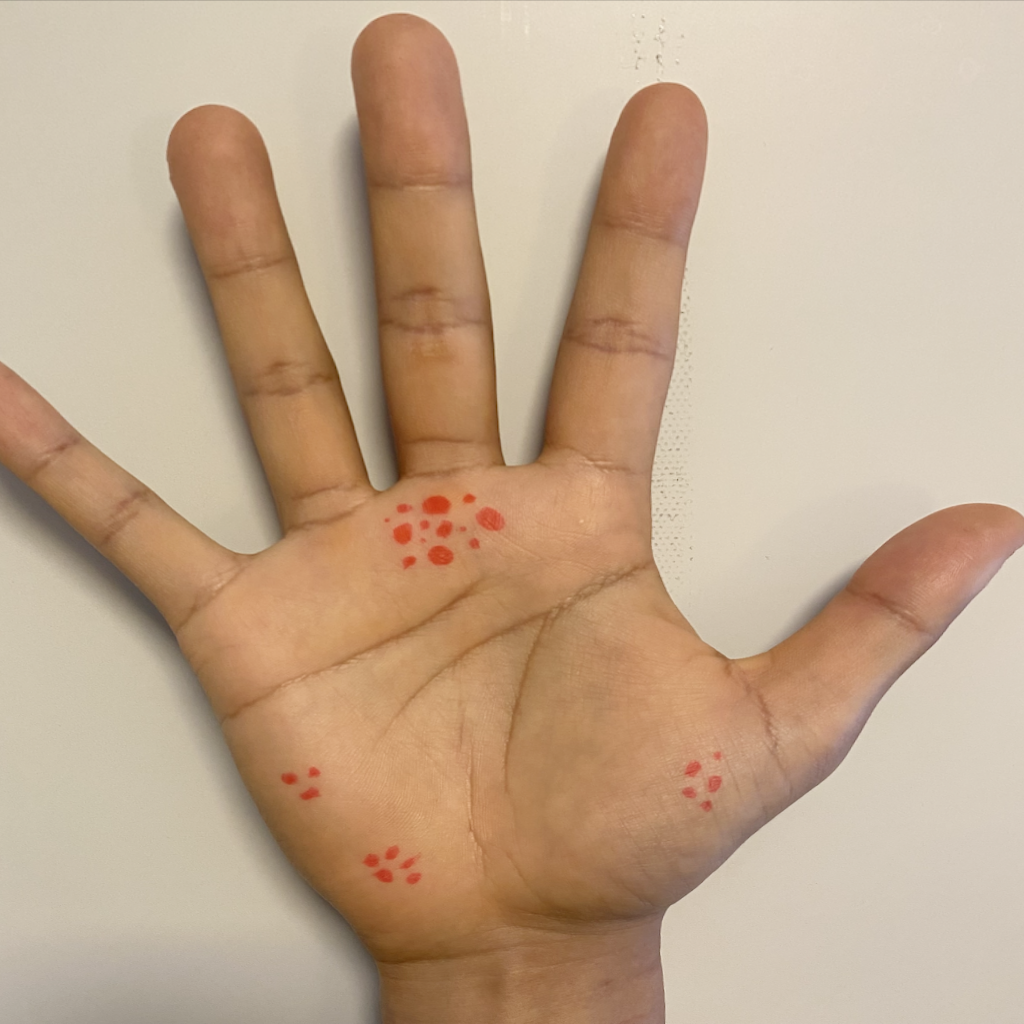
\includegraphics[width=\gridimagewidth,valign=m]{img/supplementary/orientation/perspective_bottom/0_perspective_bottom_0.2.png} & 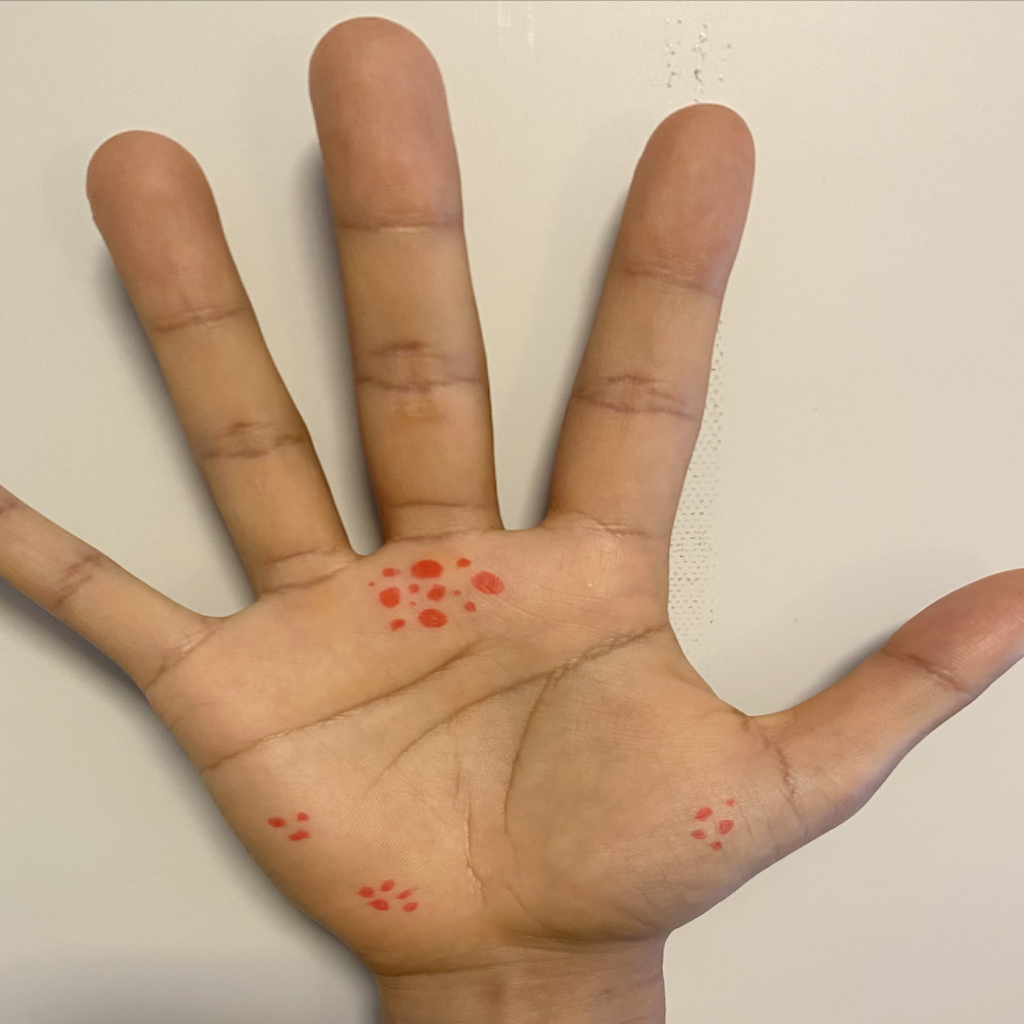
\includegraphics[width=\gridimagewidth,valign=m]{img/supplementary/orientation/perspective_bottom/0_perspective_bottom_0.4.png} & 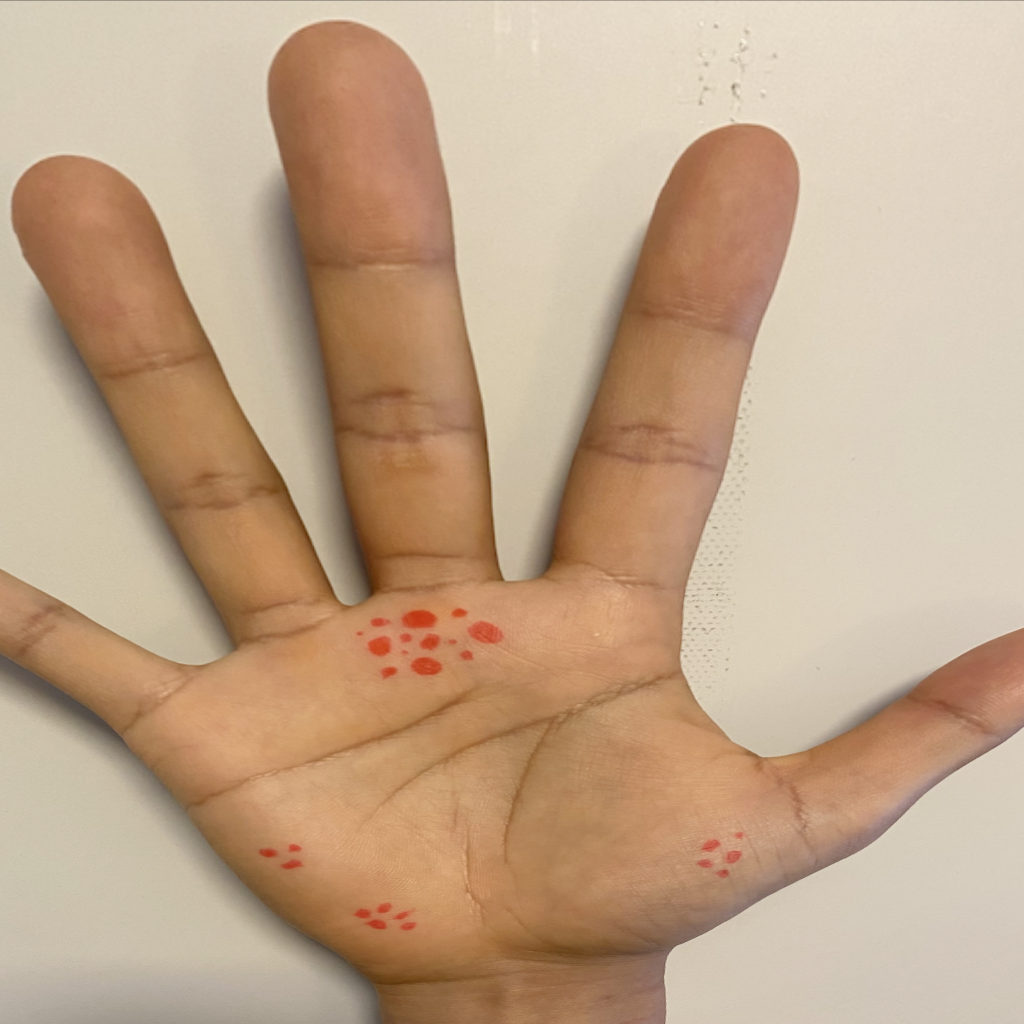
\includegraphics[width=\gridimagewidth,valign=m]{img/supplementary/orientation/perspective_bottom/0_perspective_bottom_0.6.png} & 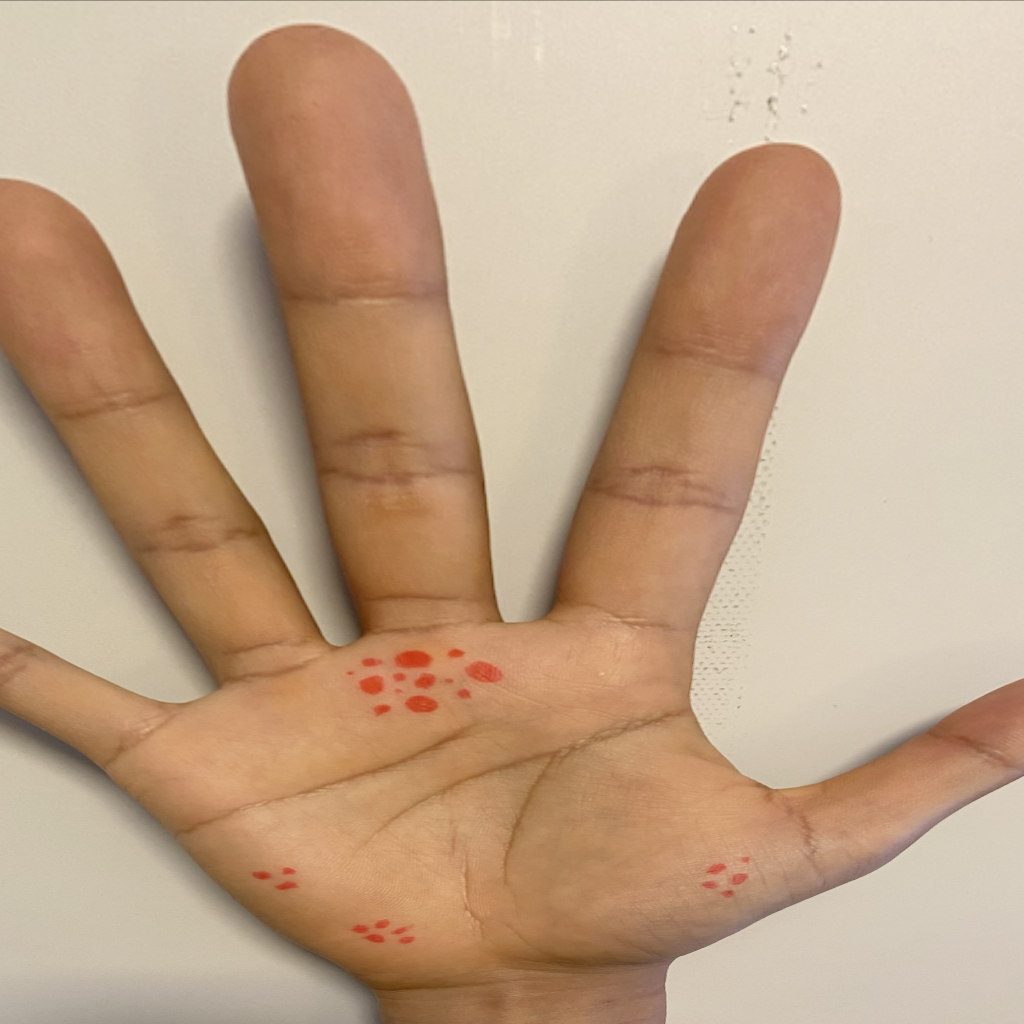
\includegraphics[width=\gridimagewidth,valign=m]{img/supplementary/orientation/perspective_bottom/0_perspective_bottom_0.8.png} \\ [6.15ex]
            Perspective top & 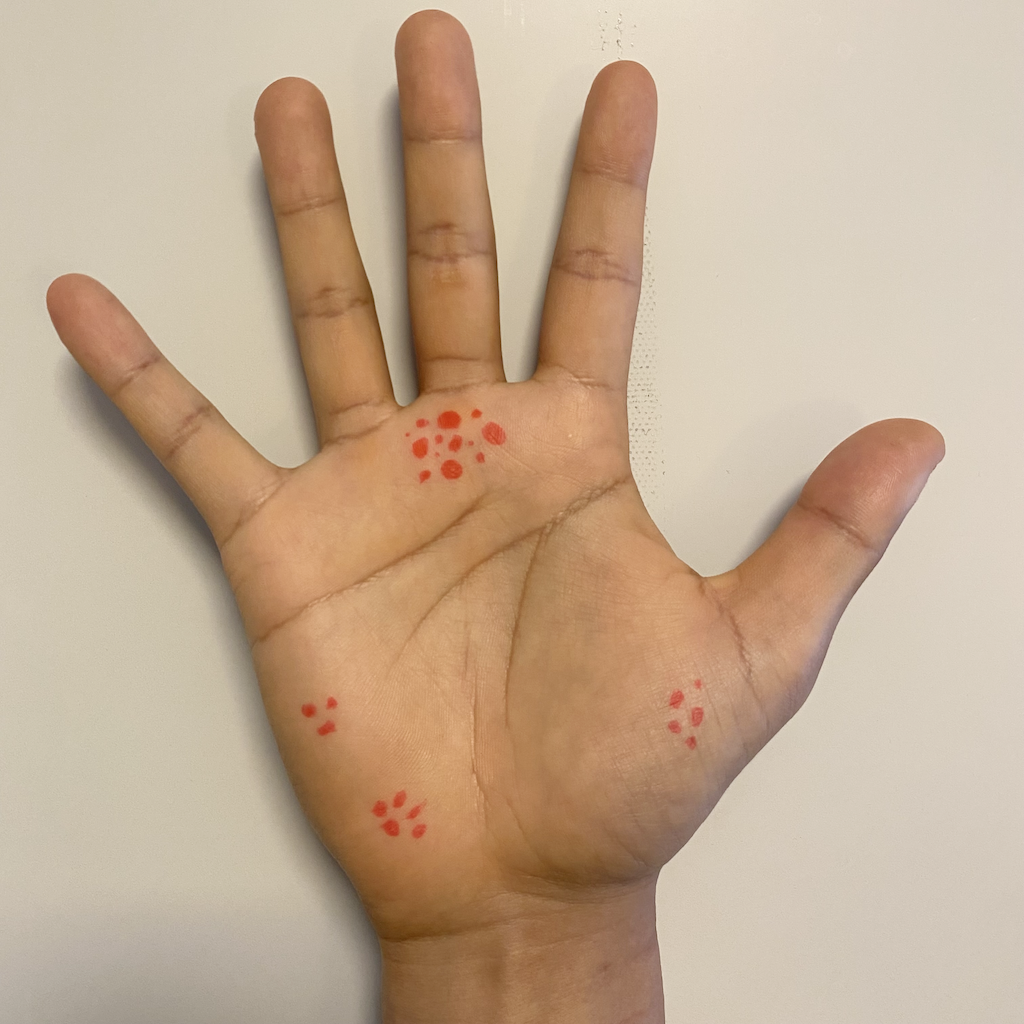
\includegraphics[width=\gridimagewidth,valign=m]{img/supplementary/orientation/perspective_top/0_perspective_top_0.0.png} & 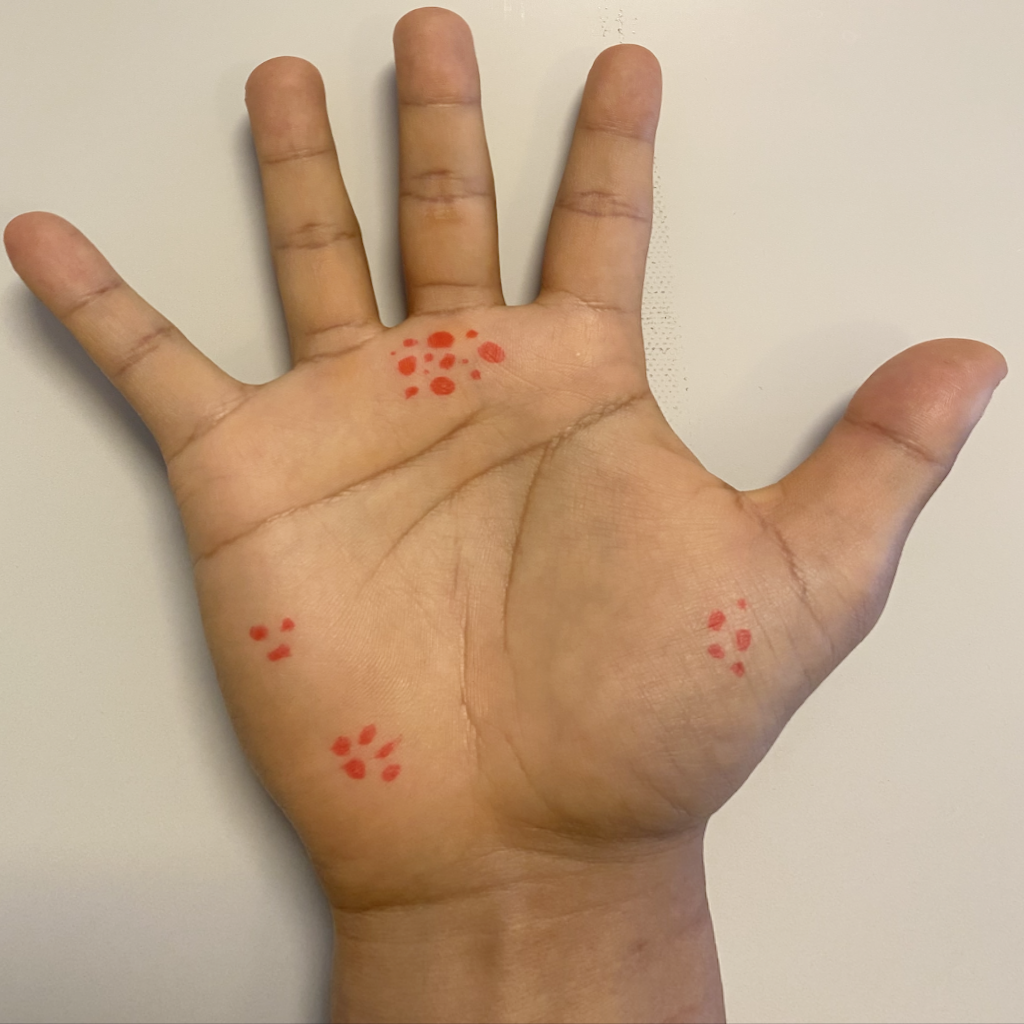
\includegraphics[width=\gridimagewidth,valign=m]{img/supplementary/orientation/perspective_top/0_perspective_top_0.2.png} & 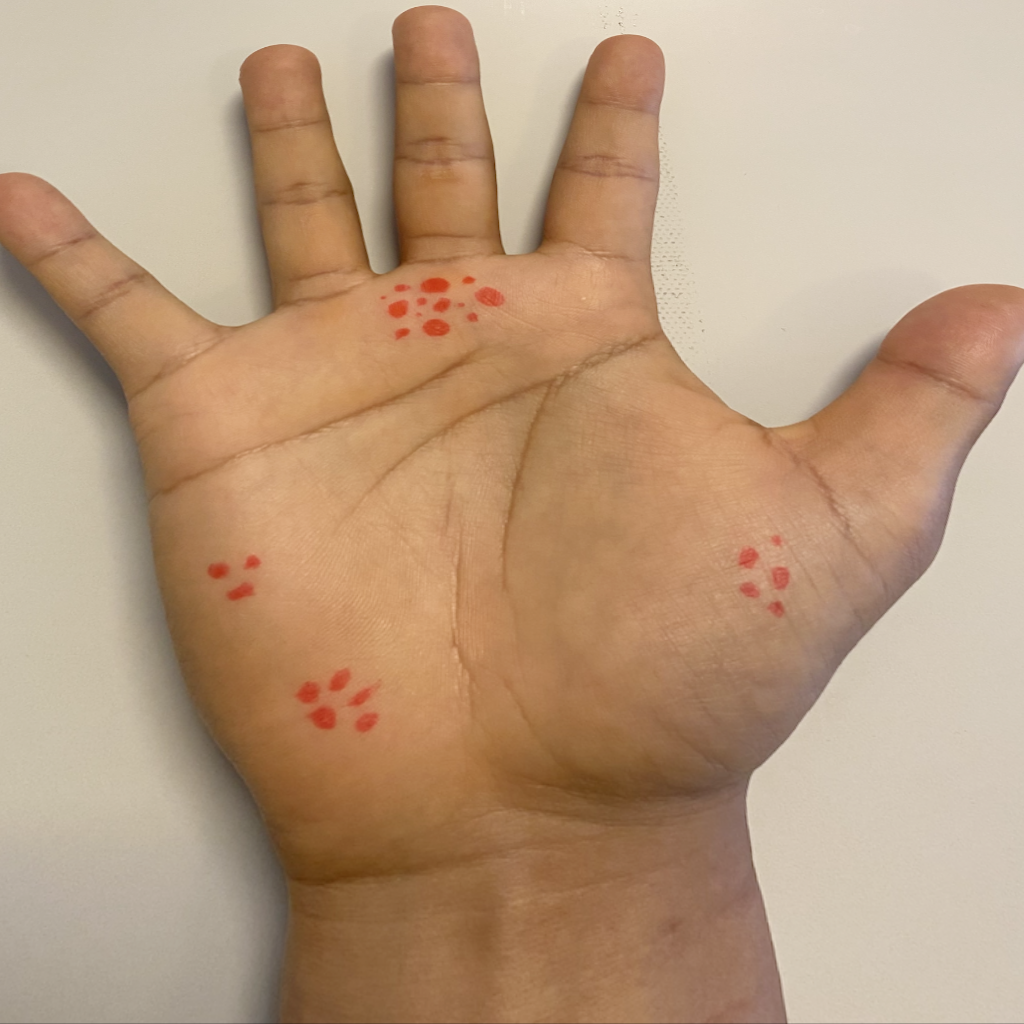
\includegraphics[width=\gridimagewidth,valign=m]{img/supplementary/orientation/perspective_top/0_perspective_top_0.4.png} & 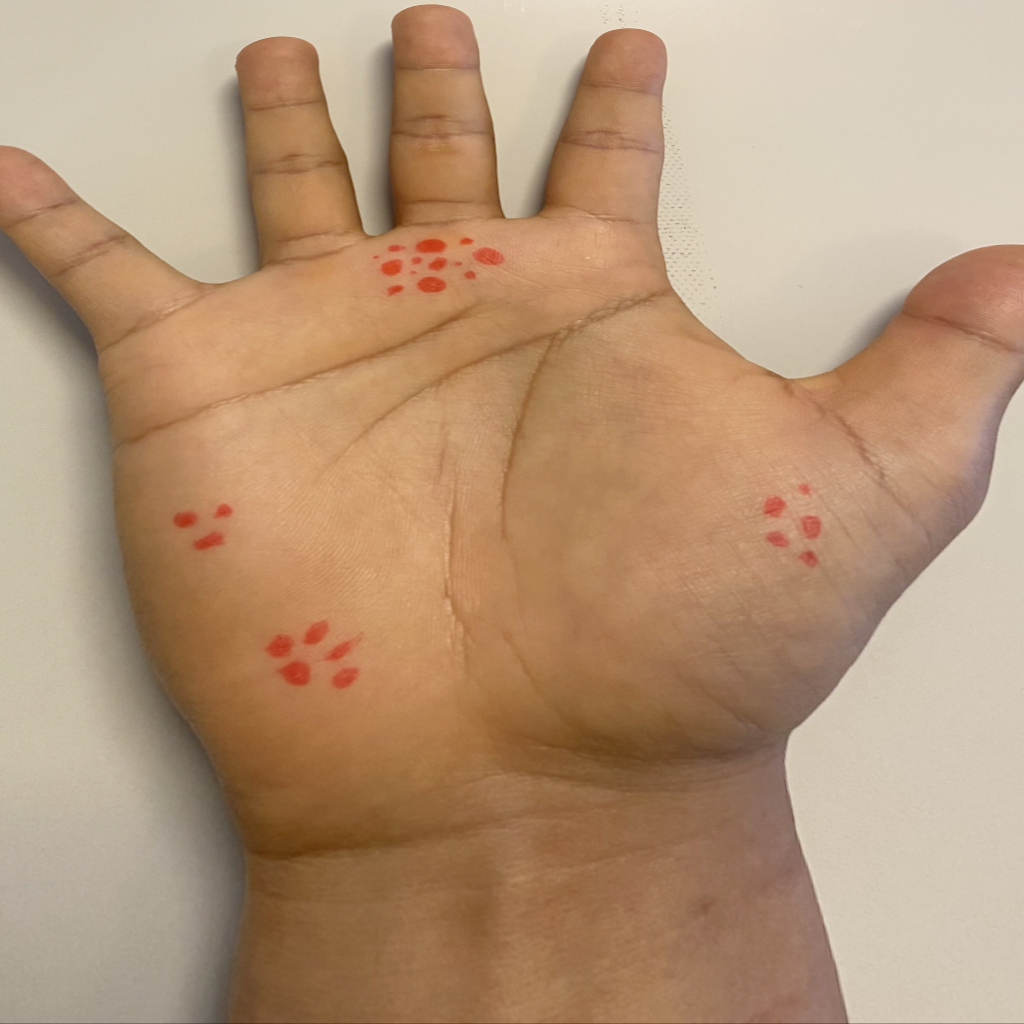
\includegraphics[width=\gridimagewidth,valign=m]{img/supplementary/orientation/perspective_top/0_perspective_top_0.6.png} & 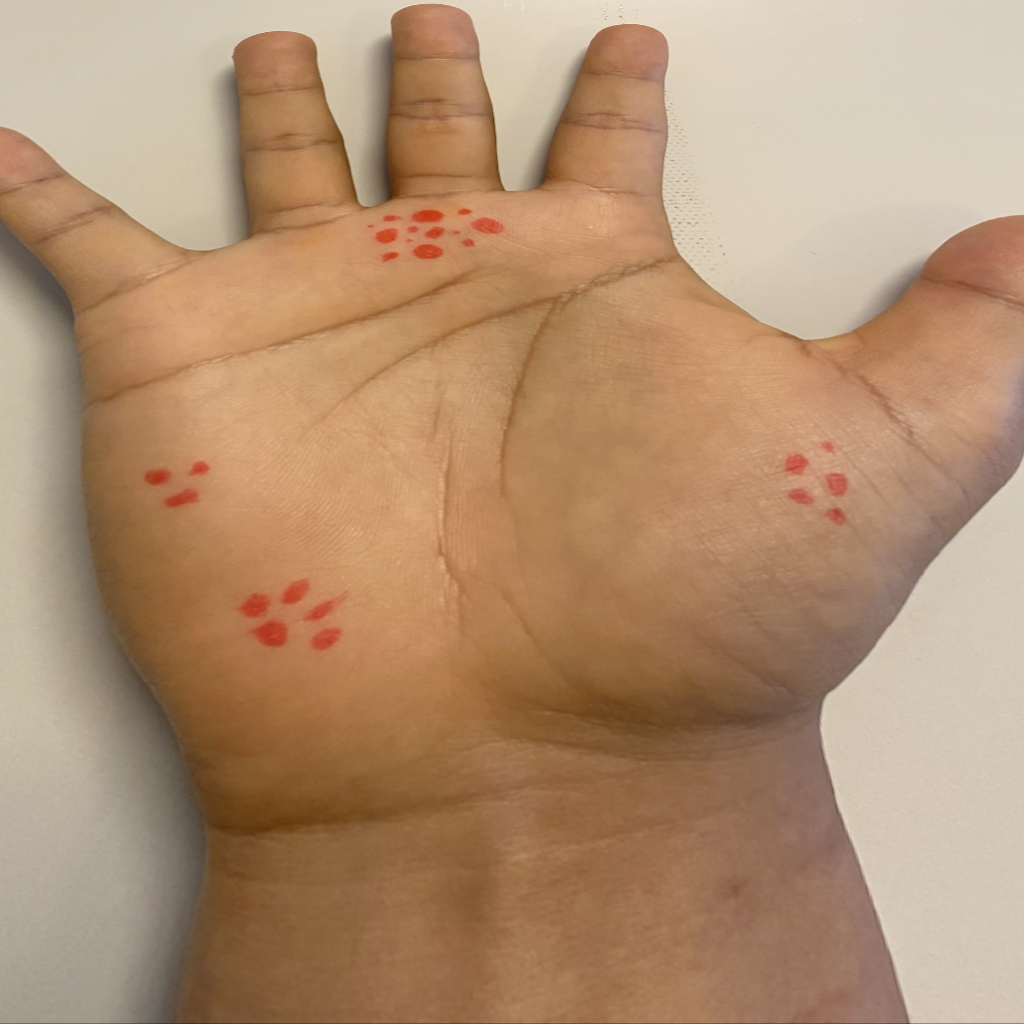
\includegraphics[width=\gridimagewidth,valign=m]{img/supplementary/orientation/perspective_top/0_perspective_top_0.8.png} \\ [6.15ex]
            Perspective left & 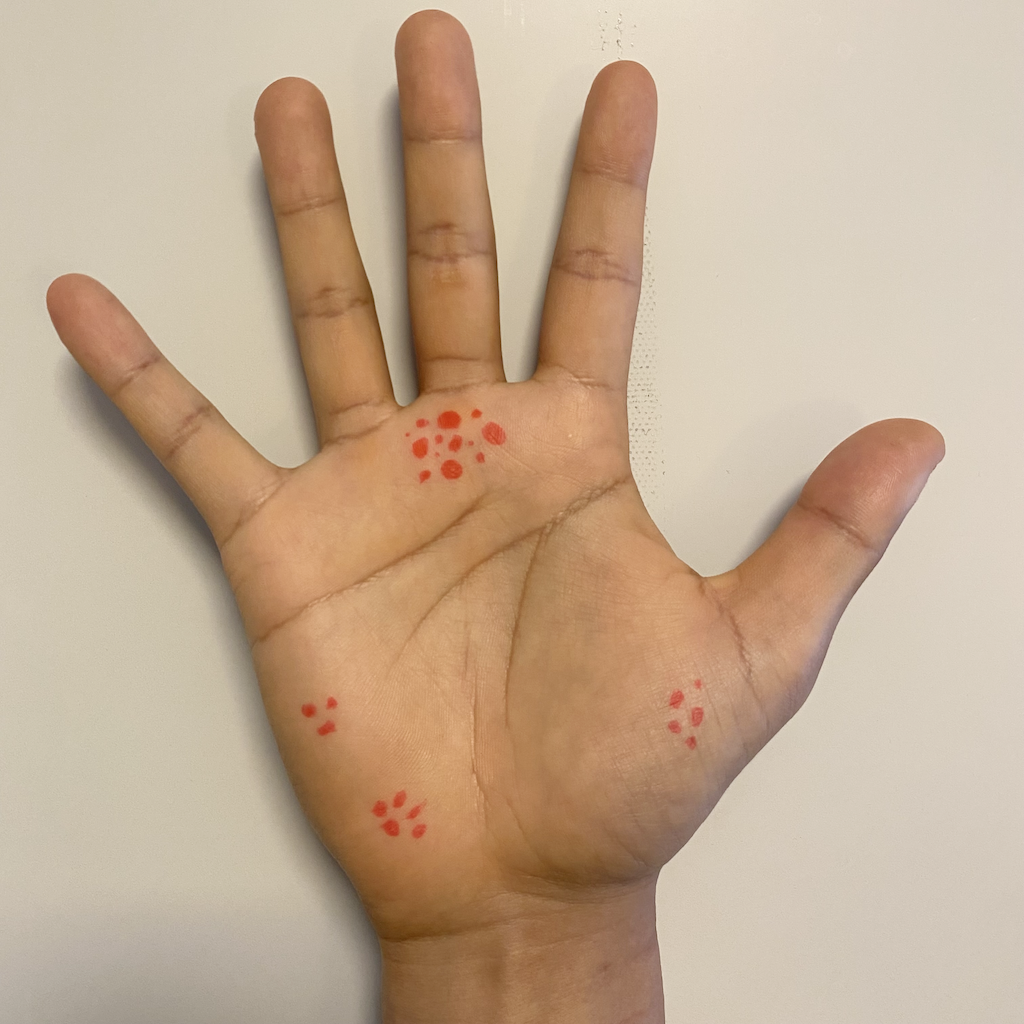
\includegraphics[width=\gridimagewidth,valign=m]{img/supplementary/orientation/perspective_left/0_perspective_left_0.0.png} & 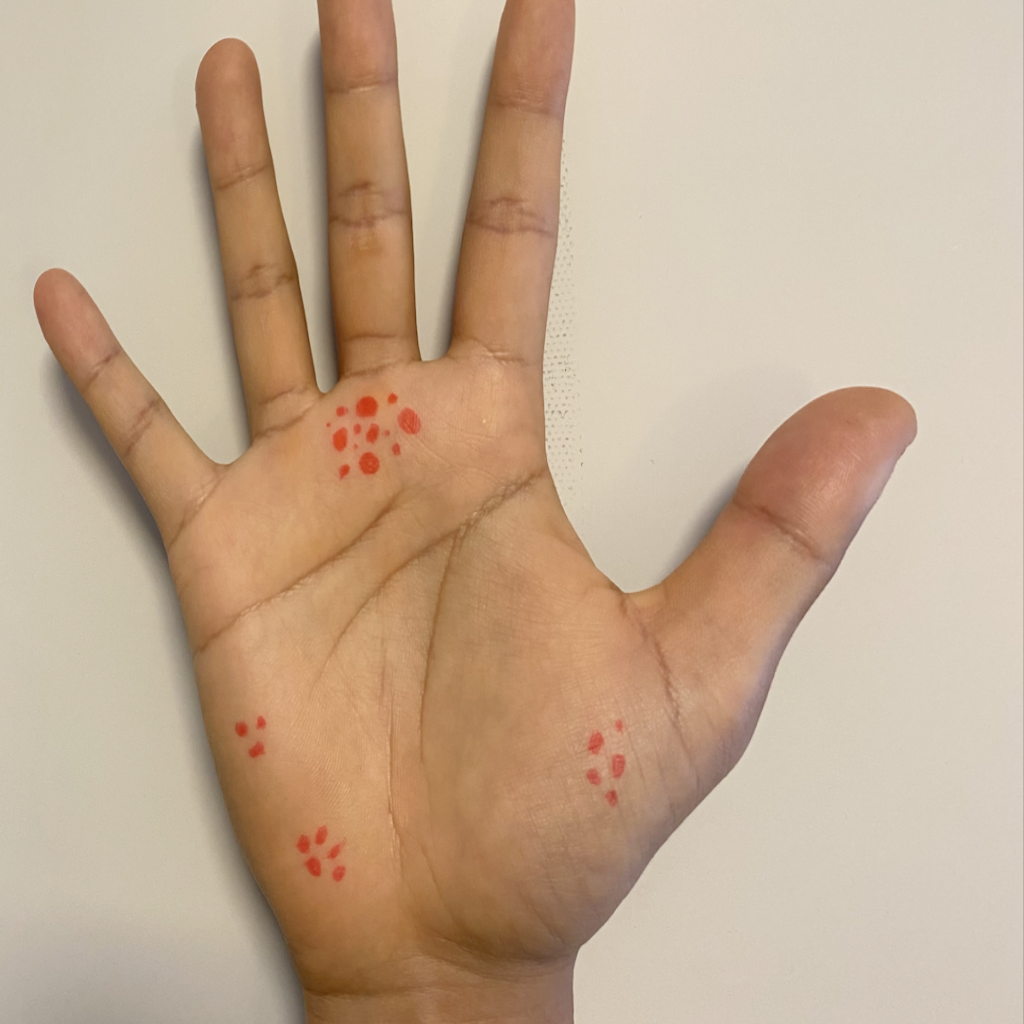
\includegraphics[width=\gridimagewidth,valign=m]{img/supplementary/orientation/perspective_left/0_perspective_left_0.2.png} & 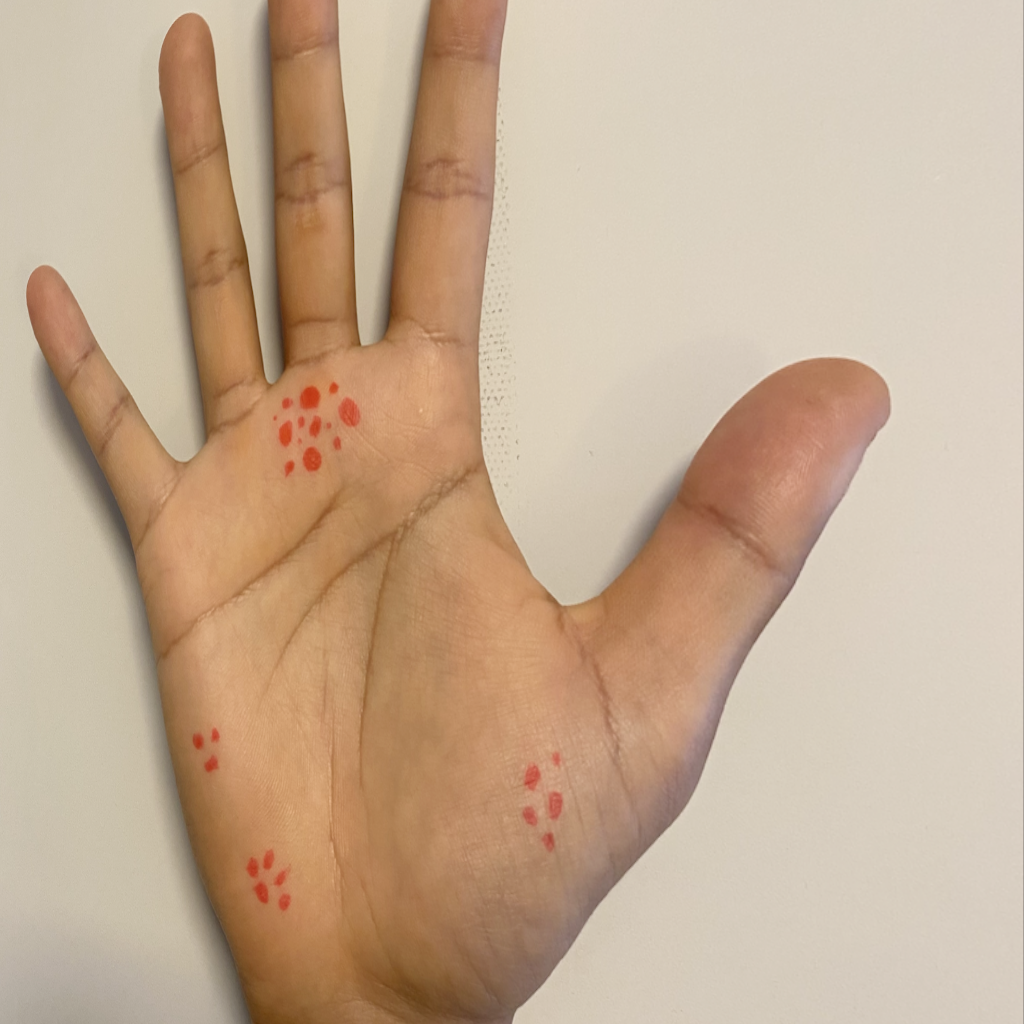
\includegraphics[width=\gridimagewidth,valign=m]{img/supplementary/orientation/perspective_left/0_perspective_left_0.4.png} & 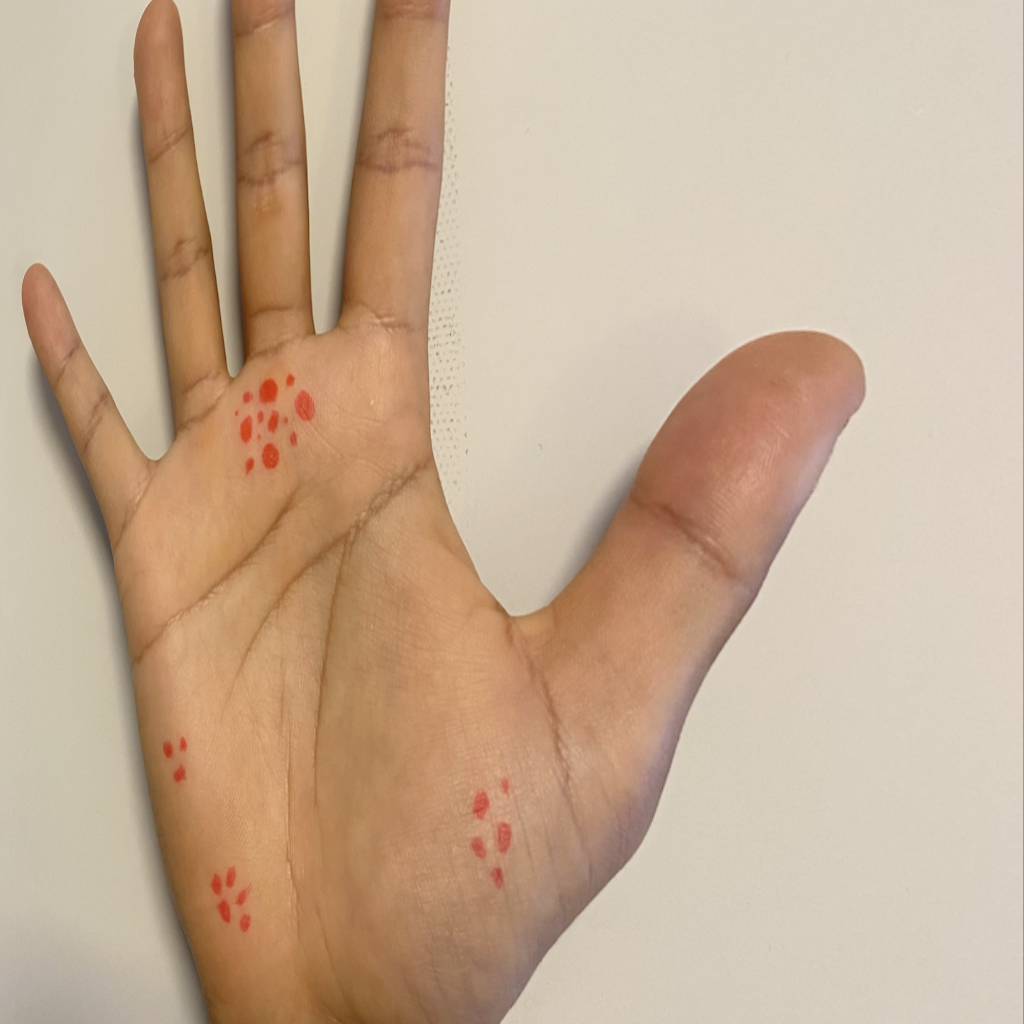
\includegraphics[width=\gridimagewidth,valign=m]{img/supplementary/orientation/perspective_left/0_perspective_left_0.6.png} & 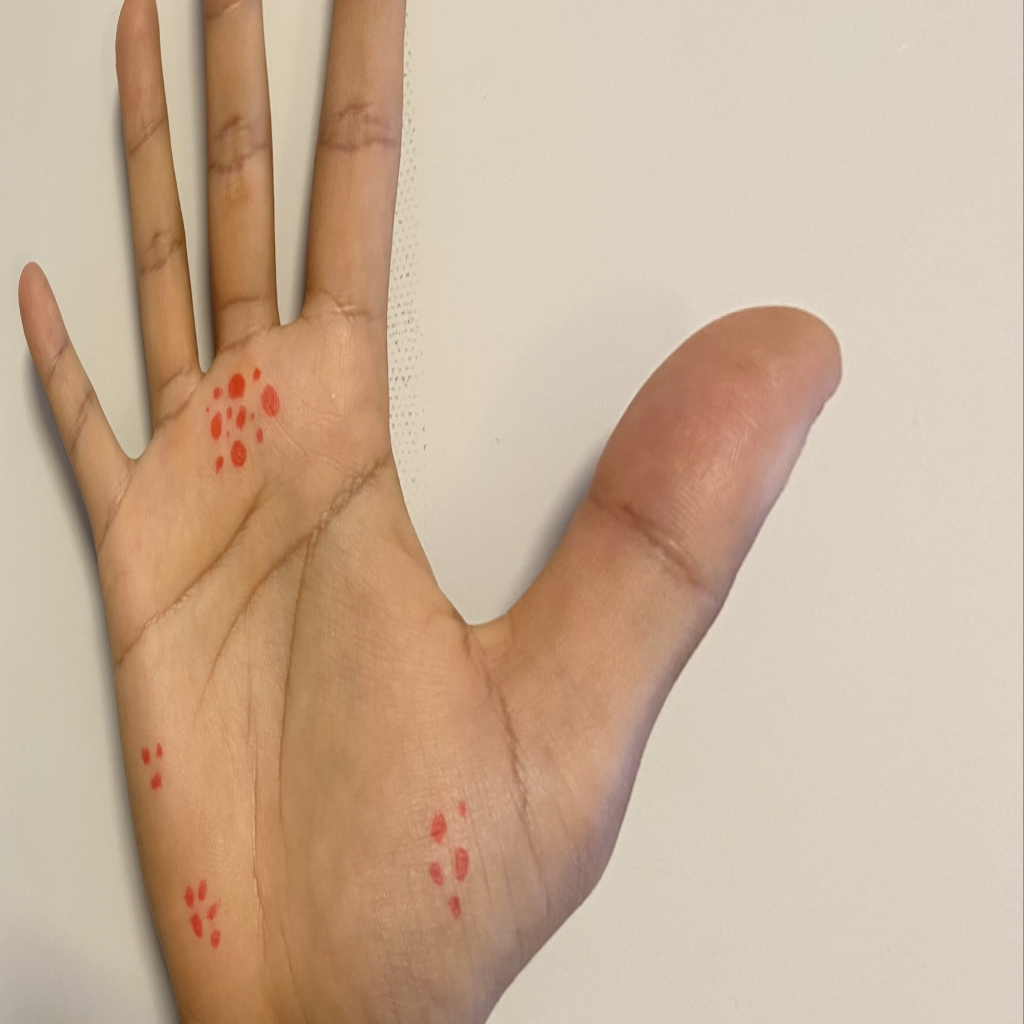
\includegraphics[width=\gridimagewidth,valign=m]{img/supplementary/orientation/perspective_left/0_perspective_left_0.8.png} \\ [6.15ex]
            Perspective right & 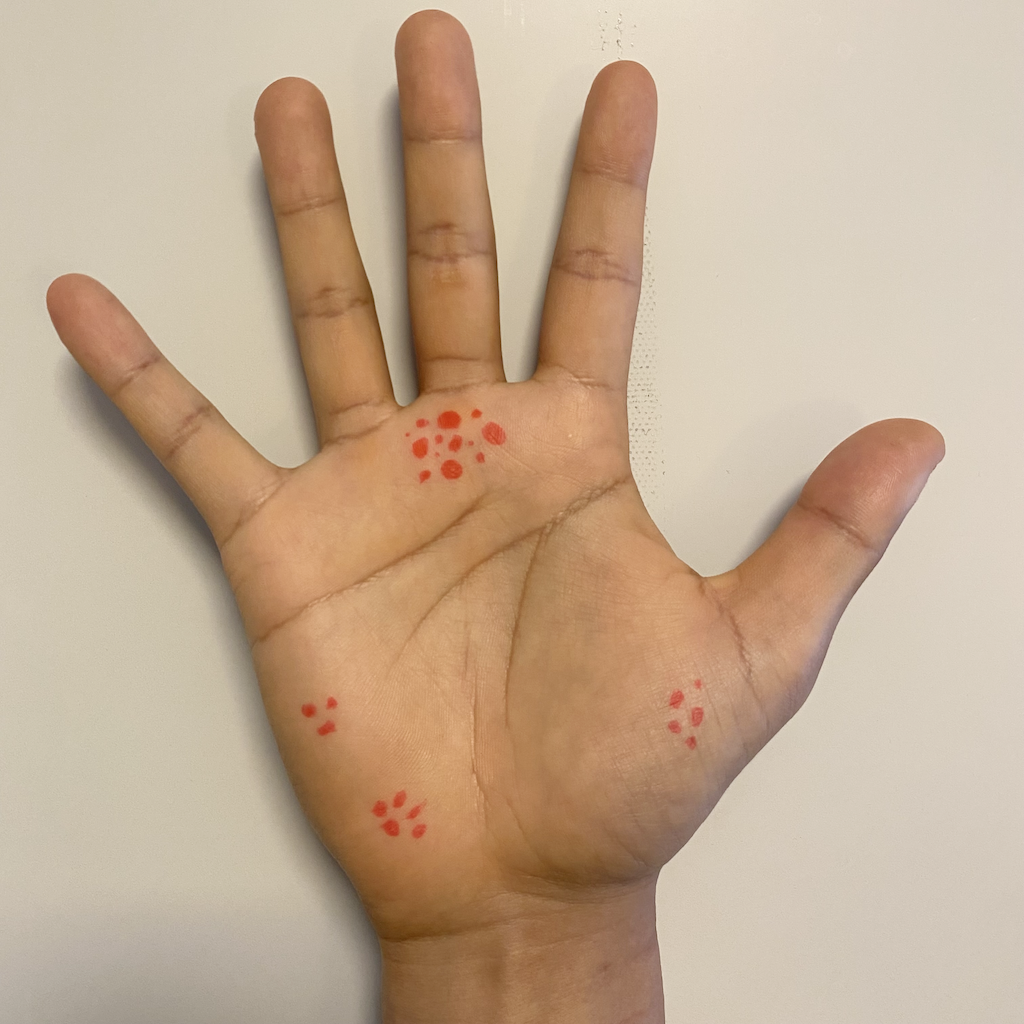
\includegraphics[width=\gridimagewidth,valign=m]{img/supplementary/orientation/perspective_right/0_perspective_right_0.0.png} & 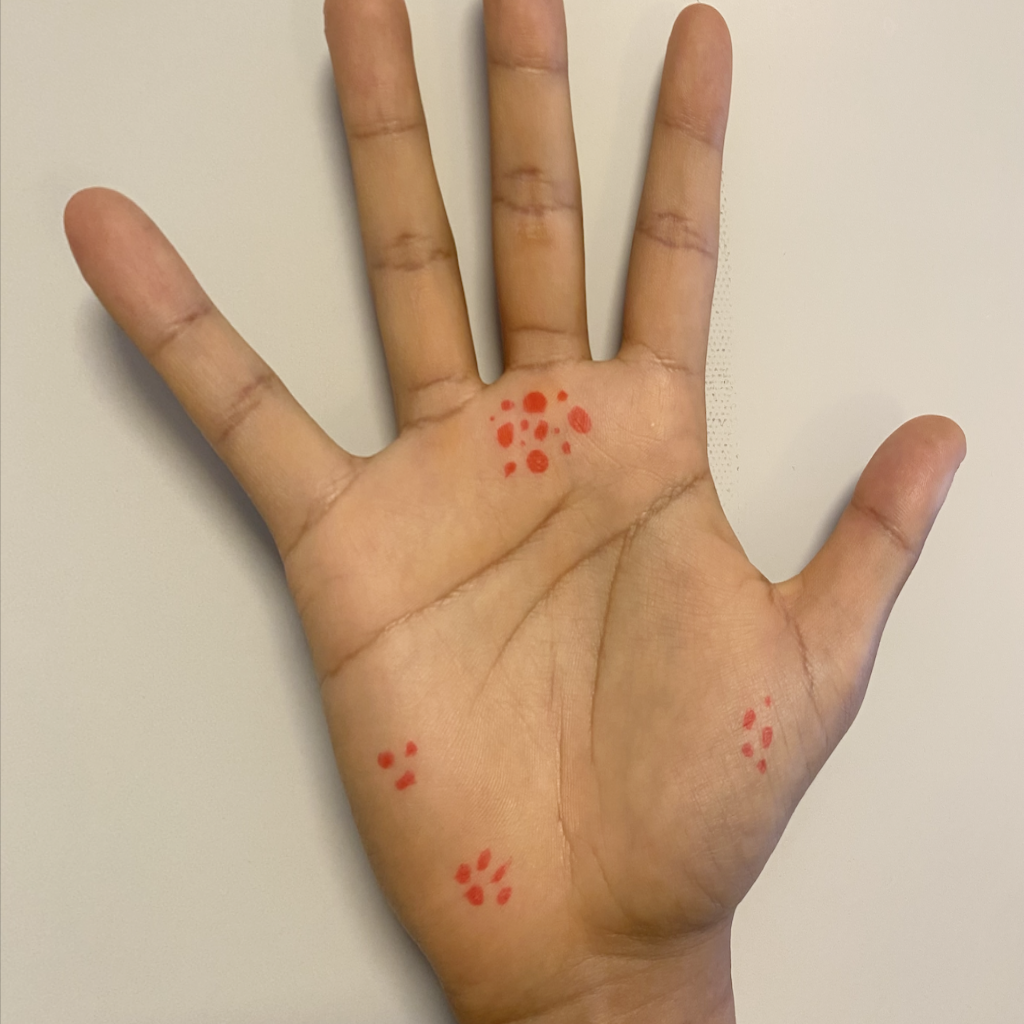
\includegraphics[width=\gridimagewidth,valign=m]{img/supplementary/orientation/perspective_right/0_perspective_right_0.2.png} & 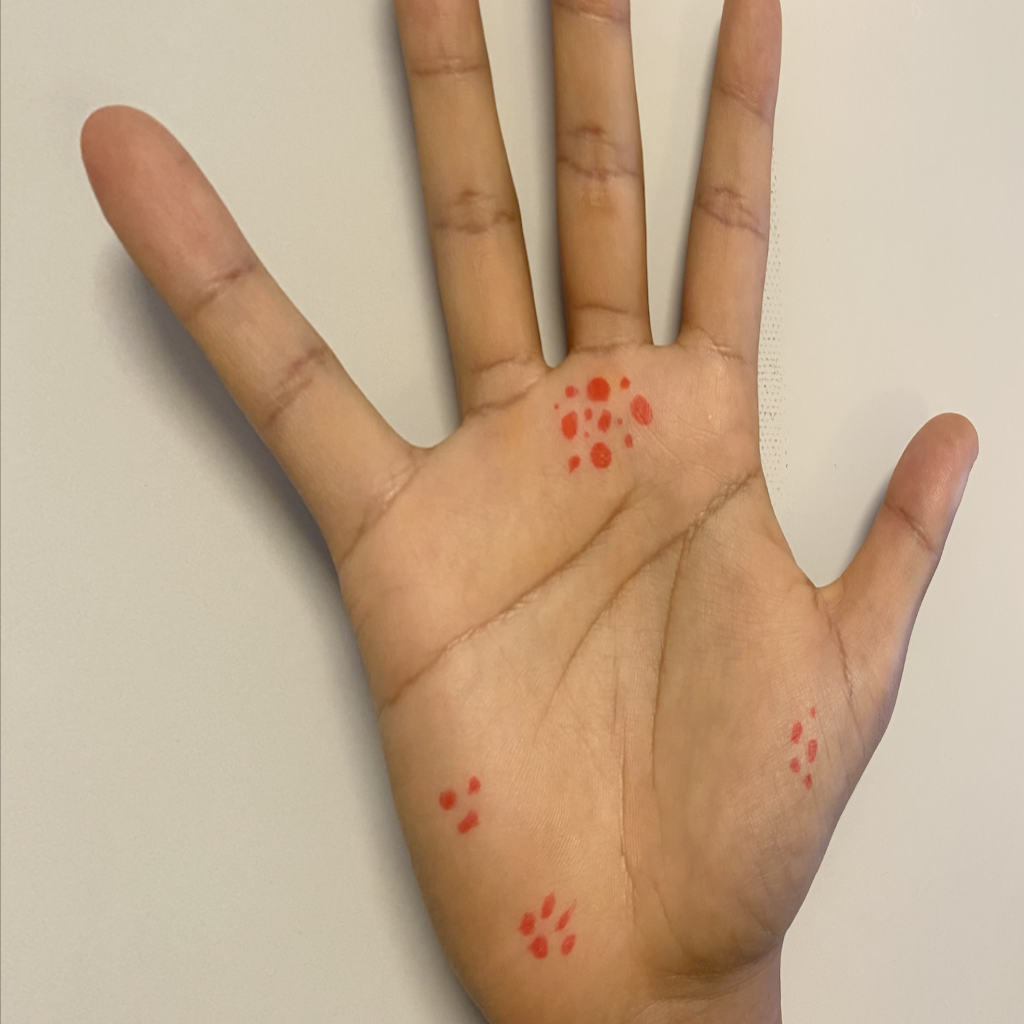
\includegraphics[width=\gridimagewidth,valign=m]{img/supplementary/orientation/perspective_right/0_perspective_right_0.4.png} & 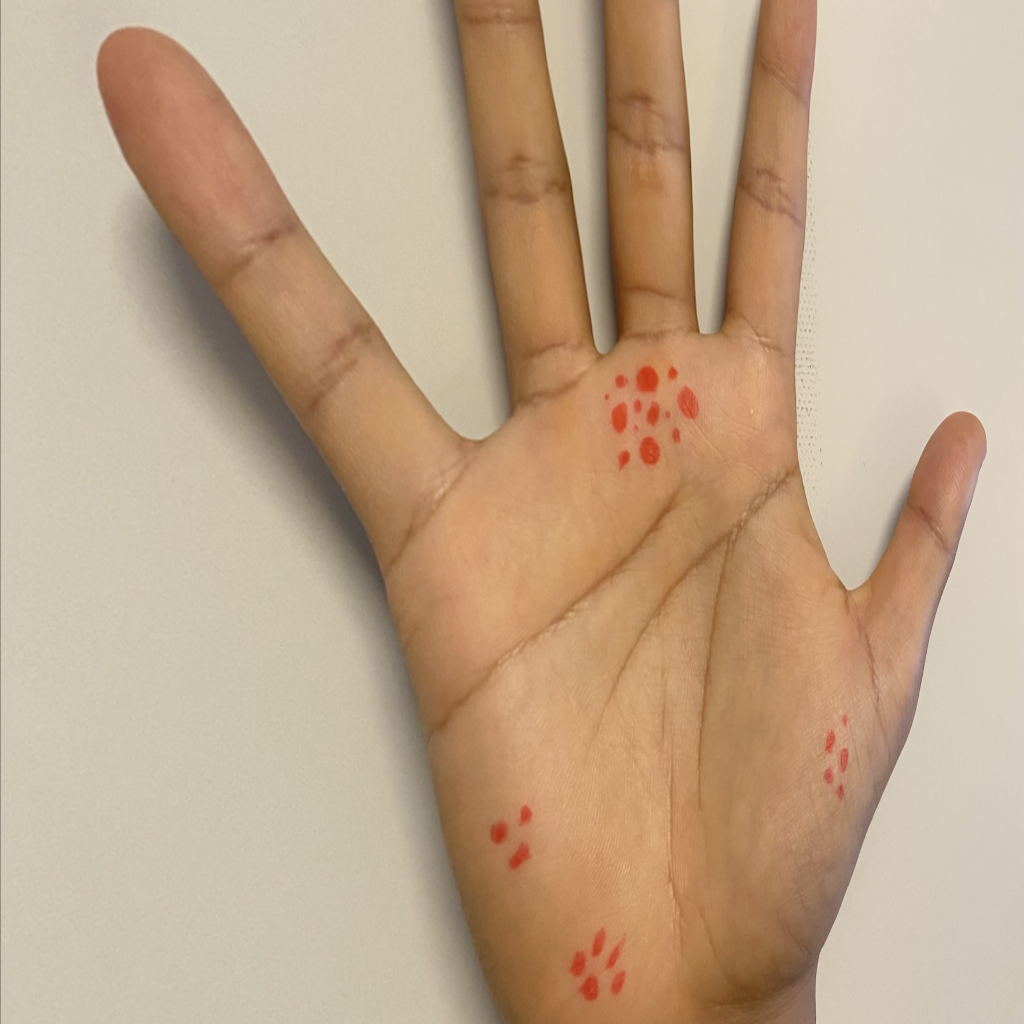
\includegraphics[width=\gridimagewidth,valign=m]{img/supplementary/orientation/perspective_right/0_perspective_right_0.6.png} & 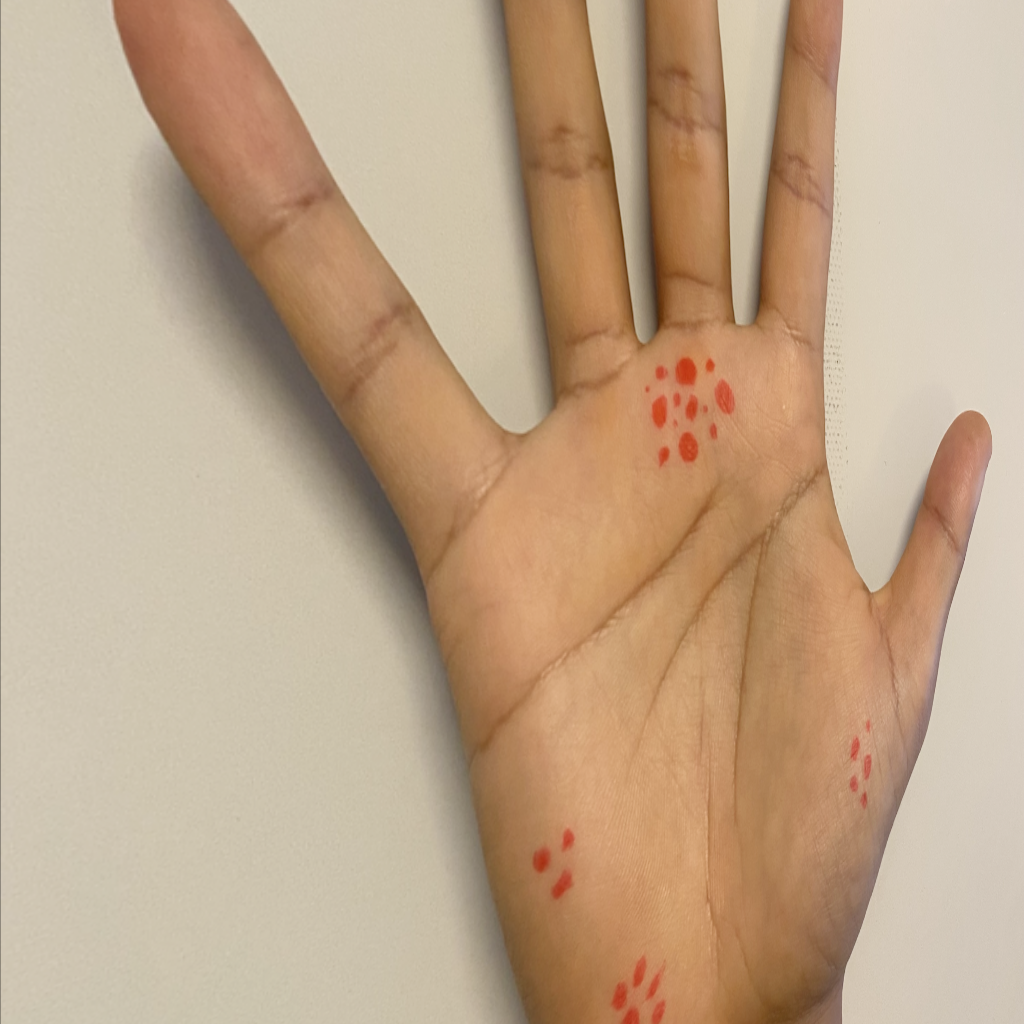
\includegraphics[width=\gridimagewidth,valign=m]{img/supplementary/orientation/perspective_right/0_perspective_right_0.8.png} \\ [6.15ex]
        \end{tabular}
    }
    \caption{Visualization of the degradation types belonging to the \textit{Image orientation} group for increasing levels of intensity.}
    \label{fig:orientation_supplementary}
\end{figure*}

\begin{figure*}[ht]
    \centering
    \setlength{\tabcolsep}{1pt}
    \Large
    \resizebox{\textwidth}{!}{%
        \begin{tabular}{C{5em}ccccc}
            & Level 1 & Level 2 & Level 3 & Level 4 & Level 5 \\
            Gaussian blur & 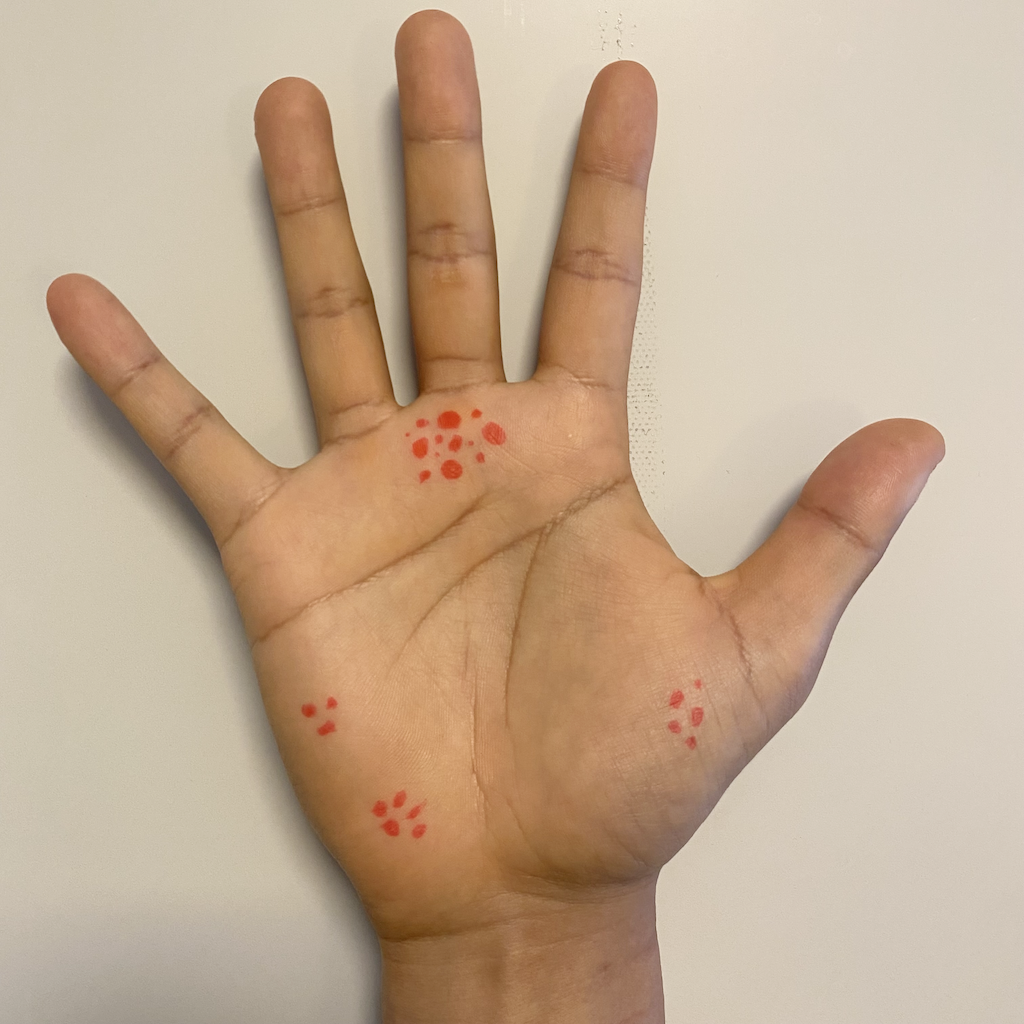
\includegraphics[width=\gridimagewidth,valign=m]{img/supplementary/focus/gaussian_blur/0_gaussian_blur_0.png} & 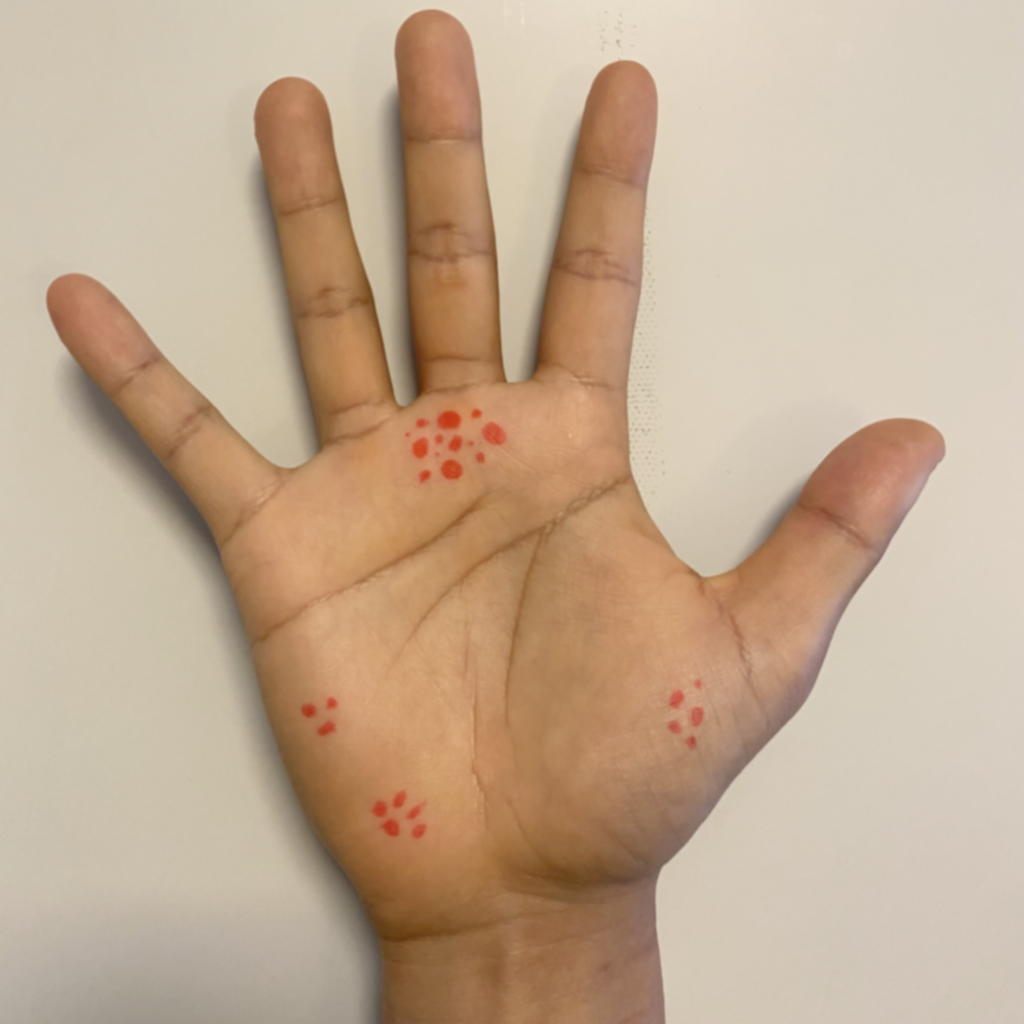
\includegraphics[width=\gridimagewidth,valign=m]{img/supplementary/focus/gaussian_blur/0_gaussian_blur_1.png} & 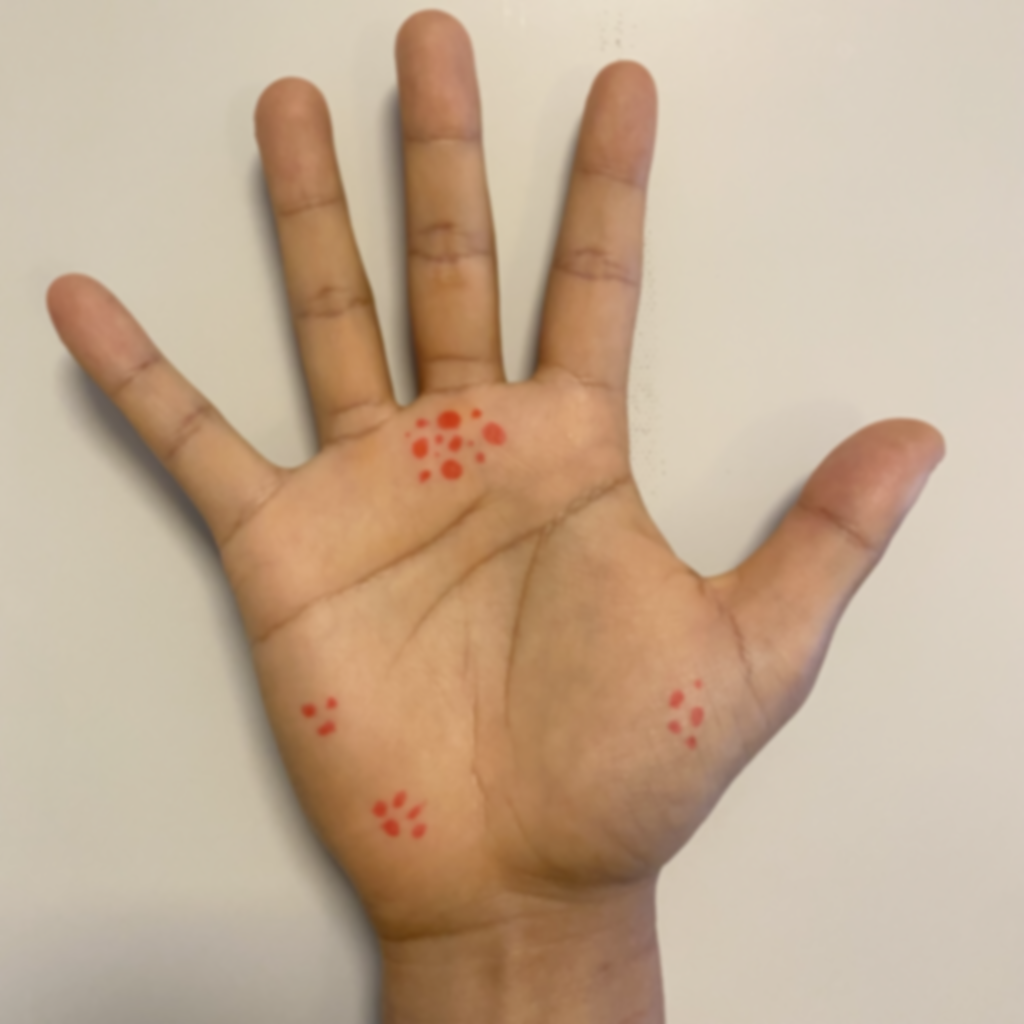
\includegraphics[width=\gridimagewidth,valign=m]{img/supplementary/focus/gaussian_blur/0_gaussian_blur_2.png} & 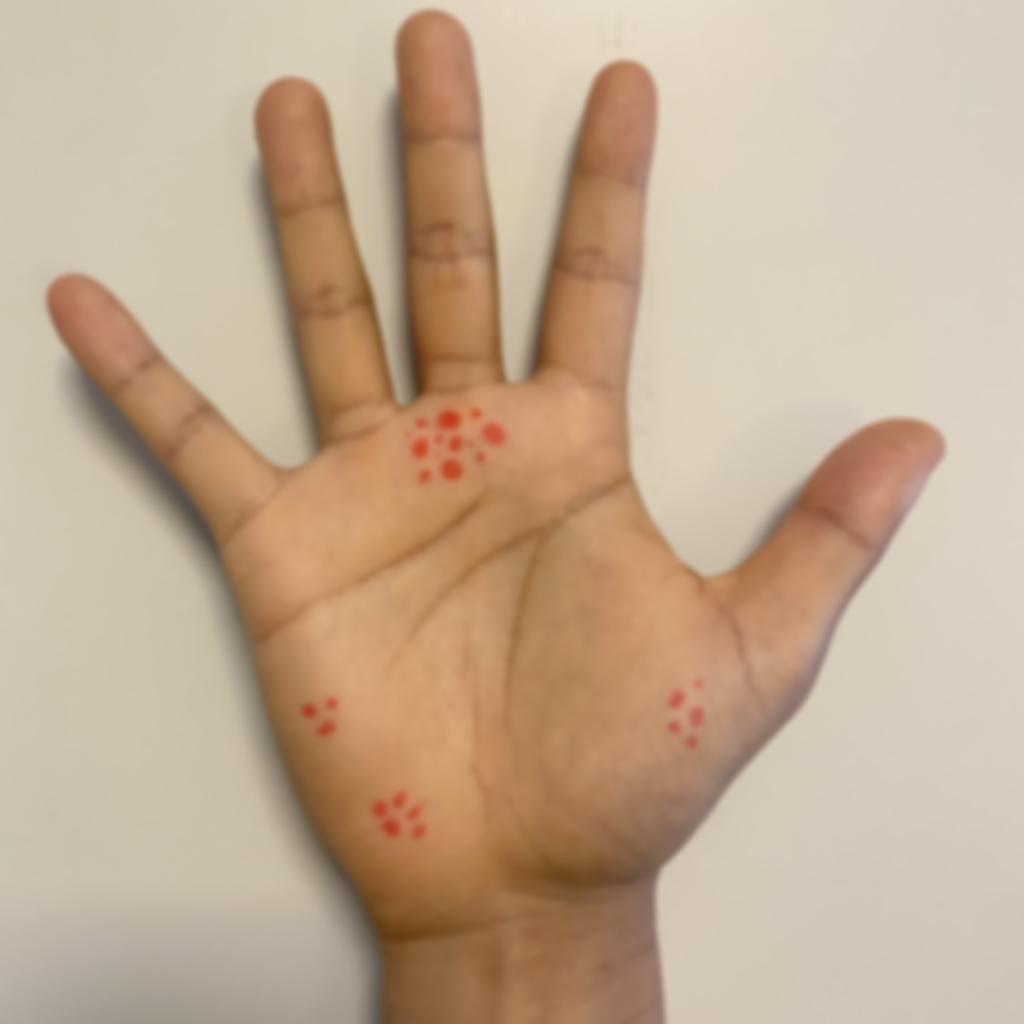
\includegraphics[width=\gridimagewidth,valign=m]{img/supplementary/focus/gaussian_blur/0_gaussian_blur_3.png} & 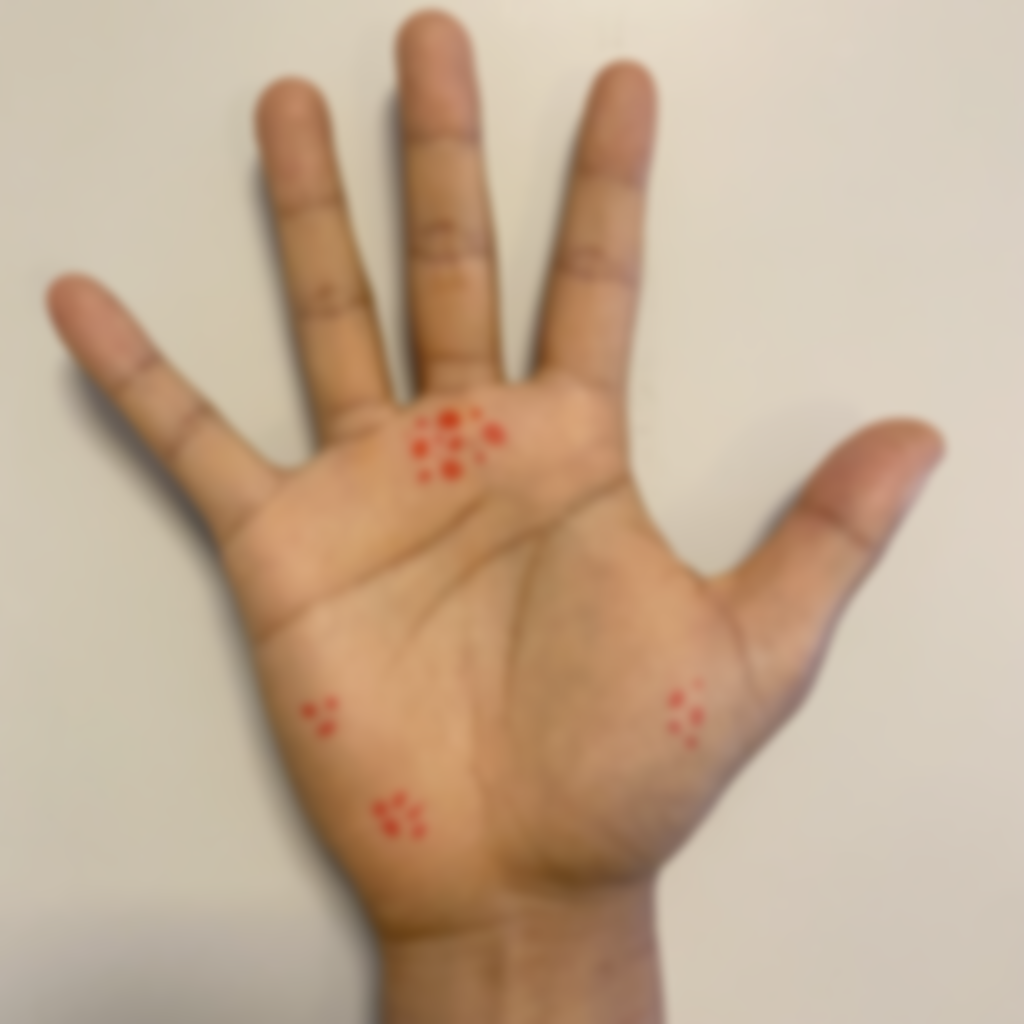
\includegraphics[width=\gridimagewidth,valign=m]{img/supplementary/focus/gaussian_blur/0_gaussian_blur_5.png} \\ [6.15ex]
            Lens blur & 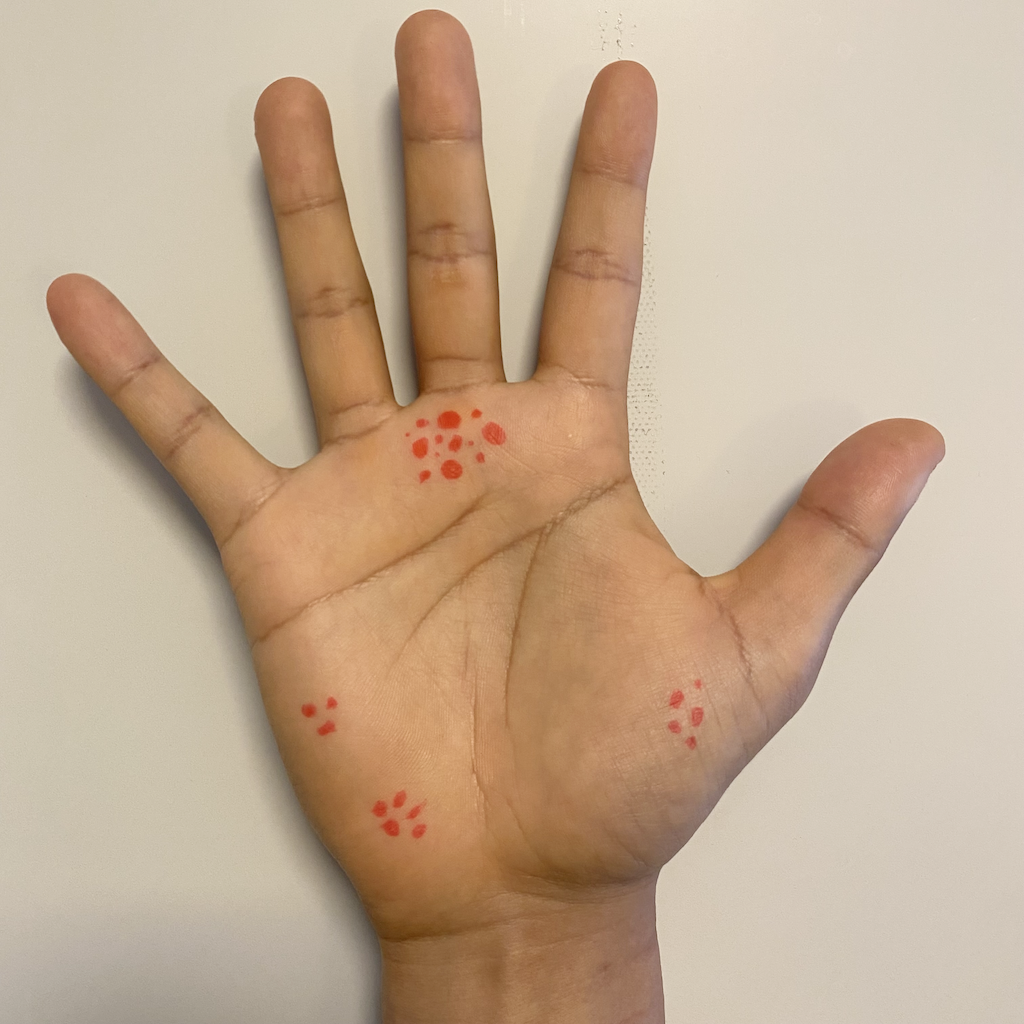
\includegraphics[width=\gridimagewidth,valign=m]{img/supplementary/focus/lens_blur/0_lens_blur_0.png} & 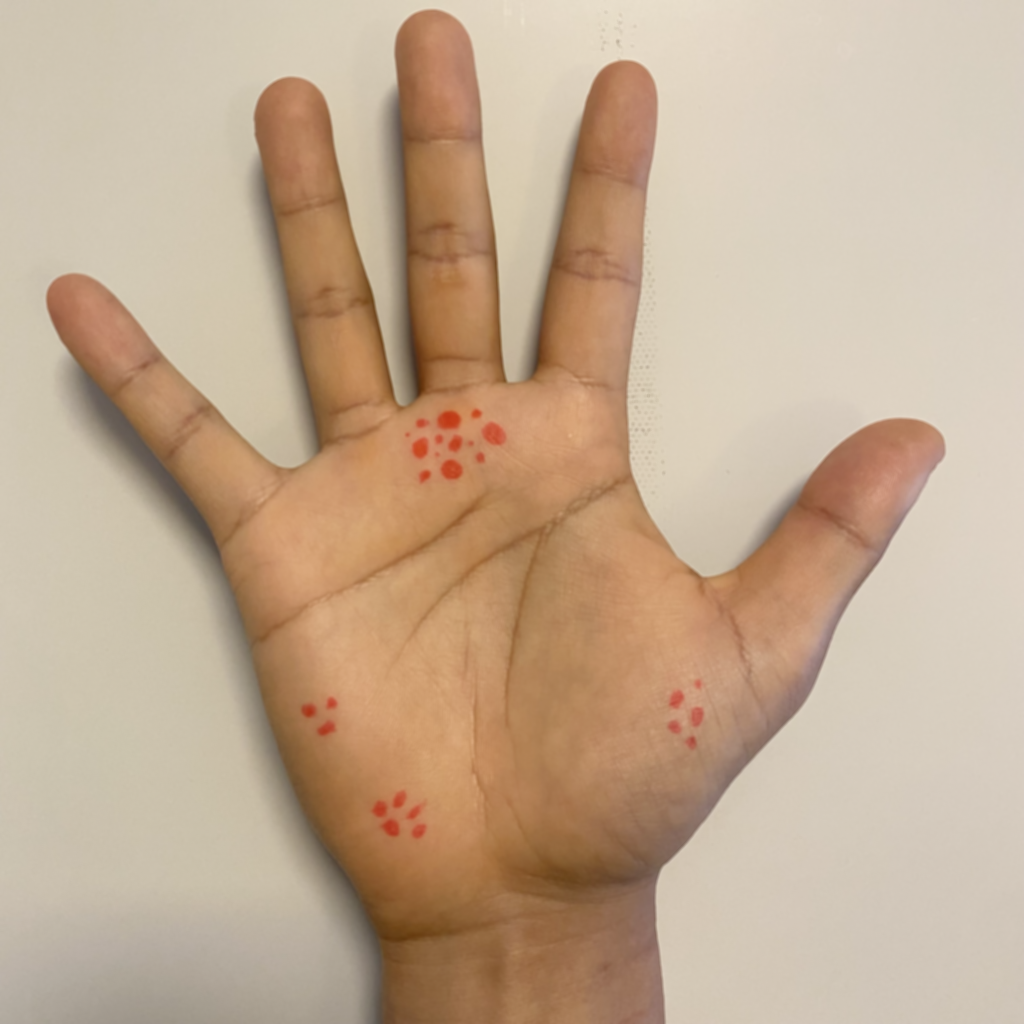
\includegraphics[width=\gridimagewidth,valign=m]{img/supplementary/focus/lens_blur/0_lens_blur_2.png} & \includegraphics[width=\gridimagewidth,valign=m]{img/supplementary/focus/lens_blur/0_lens_blur_4.png} & \includegraphics[width=\gridimagewidth,valign=m]{img/supplementary/focus/lens_blur/0_lens_blur_6.png} & \includegraphics[width=\gridimagewidth,valign=m]{img/supplementary/focus/lens_blur/0_lens_blur_8.png} \\ [6.15ex]
            Motion blur & \includegraphics[width=\gridimagewidth,valign=m]{img/supplementary/focus/motion_blur/0_motion_blur_0.png} & \includegraphics[width=\gridimagewidth,valign=m]{img/supplementary/focus/motion_blur/0_motion_blur_2.png} & \includegraphics[width=\gridimagewidth,valign=m]{img/supplementary/focus/motion_blur/0_motion_blur_4.png} & \includegraphics[width=\gridimagewidth,valign=m]{img/supplementary/focus/motion_blur/0_motion_blur_6.png} & \includegraphics[width=\gridimagewidth,valign=m]{img/supplementary/focus/motion_blur/0_motion_blur_8.png} \\ [6.15ex]
        \end{tabular}
    }
    \caption{Visualization of the degradation types belonging to the \textit{Focus} group for increasing levels of intensity.}
    \label{fig:focus_supplementary}
\end{figure*}

\begin{figure*}[ht]
    \centering
    \setlength{\tabcolsep}{1pt}
    \Large
    \resizebox{\textwidth}{!}{%
        \begin{tabular}{C{5em}ccccc}
            & Level 1 & Level 2 & Level 3 & Level 4 & Level 5 \\
            Change resolution & \includegraphics[width=\gridimagewidth,valign=m]{img/supplementary/resolution/change_resolution/0_change_resolution_0.0.png} & \includegraphics[width=\gridimagewidth,valign=m]{img/supplementary/resolution/change_resolution/0_change_resolution_0.2.png} & \includegraphics[width=\gridimagewidth,valign=m]{img/supplementary/resolution/change_resolution/0_change_resolution_0.4.png} & \includegraphics[width=\gridimagewidth,valign=m]{img/supplementary/resolution/change_resolution/0_change_resolution_0.6.png} & \includegraphics[width=\gridimagewidth,valign=m]{img/supplementary/resolution/change_resolution/0_change_resolution_0.8.png} \\ [6.15ex]
        \end{tabular}
    }
    \caption{Visualization of the degradation types belonging to the \textit{Resolution} group for increasing levels of intensity.}
    \label{fig:resolution_supplementary}
\end{figure*}

\begin{figure*}[ht]
    \centering
    \setlength{\tabcolsep}{1pt}
    \Large
    \resizebox{\textwidth}{!}{%
        \begin{tabular}{C{5em}ccccc}
            & Level 1 & Level 2 & Level 3 & Level 4 & Level 5 \\
            Color saturation 1 & \includegraphics[width=\gridimagewidth,valign=m]{img/supplementary/color_calibration/color_saturation1/0_color_saturation1_0.png} & \includegraphics[width=\gridimagewidth,valign=m]{img/supplementary/color_calibration/color_saturation1/0_color_saturation1_0.2.png} & \includegraphics[width=\gridimagewidth,valign=m]{img/supplementary/color_calibration/color_saturation1/0_color_saturation1_0.4.png} & \includegraphics[width=\gridimagewidth,valign=m]{img/supplementary/color_calibration/color_saturation1/0_color_saturation1_0.6.png} & \includegraphics[width=\gridimagewidth,valign=m]{img/supplementary/color_calibration/color_saturation1/0_color_saturation1_0.8.png} \\ [6.15ex]
            Color saturation 2 & \includegraphics[width=\gridimagewidth,valign=m]{img/supplementary/color_calibration/color_saturation2/0_color_saturation2_0.png} & \includegraphics[width=\gridimagewidth,valign=m]{img/supplementary/color_calibration/color_saturation2/0_color_saturation2_1.png} & \includegraphics[width=\gridimagewidth,valign=m]{img/supplementary/color_calibration/color_saturation2/0_color_saturation2_2.png} & \includegraphics[width=\gridimagewidth,valign=m]{img/supplementary/color_calibration/color_saturation2/0_color_saturation2_3.png} & \includegraphics[width=\gridimagewidth,valign=m]{img/supplementary/color_calibration/color_saturation2/0_color_saturation2_4.png} \\ [6.15ex]
        \end{tabular}
    }
    \caption{Visualization of the degradation types belonging to the \textit{Color calibration} group for increasing levels of intensity.}
    \label{fig:color_calibration_supplementary}
\end{figure*}


\clearpage
\section{Proposed Framework for Automated Image Quality Assessment in Teledermatology}
\label{sec:framework}
\begin{figure}[ht]
    \centering
    \includegraphics[keepaspectratio,width=5.2cm]{img/Architecture.png}
    \caption{Overview of the proposed framework for automated image quality assessment in teledermatology. It starts with good quality input images, which go through a distortion pipeline covering seven dermatology quality criteria. The ARNIQA backbone extracts features, and a multi-output regressor predicts the seven quality criteria. The final predictions are visualized with radar charts.}
    \label{fig:Architecture}
\end{figure}

